

\chapter{METODOLOGIA}{}
\label{cap:04}

Neste capítulo, é descrito a metodologia que foi adotada no desenvolvimento do trabalho. O processo de treinamento do modelo de classificação de imagens, a descrição do banco de dados utilizado, a arquitetura e o funcionamento detalhado do modelo. Além disso, as ferramentas computacionais de \textit{software} e \textit{hardware} e, por fim, apresenta-se a metodologia escolhida para avaliar os resultados obtidos.

\section{Banco de dados}

O banco de dados foi extraído do artigo BananaLSD: \textit{A banana leaf images dataset for classification of banana leaf diseases using machine learning}~\cite{DadosArt}. Este conjunto de dados contém 937 imagens originais de folhas de bananeiras, divididas em quatro classes: Pestalotiopsis, Sigatoka, Cordana e folhas saudáveis. As imagens foram capturadas em condições naturais, utilizando três câmeras de smartphones, para que houvesse a maior diversidade possível no dataset em termos de iluminação e ângulos das fotos~\cite{DadosArt}.

Para o treinamento do modelo neste trabalho, são utilizadas apenas as classes Sigatoka e folhas saudáveis. A seleção dessas classes se deu para focar no desenvolvimento de um modelo que possa diferenciar entre folhas infectadas por Sigatoka e folhas saudáveis, já que a Sigatoka é considerada uma das doenças que causam mais prejuízos nas plantações de banana. A classe Sigatoka, no dataset original, contém 473 imagens, enquanto a classe de folhas saudáveis possui 129 imagens. 

\subsection{Processamento dos dados}
As imagens são de alta qualidade, portanto, foi necessário reduzi-las para um tamanho de 224x224 pixels, uma resolução mais apropriada para a construção do modelo. Em seguida, foi realizada a ampliação do conjunto das imagens redimensionadas. Modelos de aprendizado profundo tendem a ser mais eficientes quando as classes contêm mais amostras~\cite{DadosArt}. Um modelo treinado com imagens capturadas de apenas uma perspectiva tende a ser tendencioso. A ampliação garante diversidade no conjunto de dados e corrige o desbalanceamento de dados presente. As seguintes técnicas de ampliação foram aplicadas para aumentar o conjunto de dados bruto.

\begin{enumerate}
    \item Cortes: As imagens são cortadas em várias outras, reduzindo o tamanho e expandindo o conjunto de dados obtido. 
    \item Rotação horizontal: Normalmente rotacionar não é tão natural para RNC, mas para o caso em especifico não altera o aprendizado. A implementação desse aumento de dados é direta, simples de implementar e demonstrou sua eficácia na utilização deste trabalho~\cite{DadosArt}.
    \item Ajuste de contraste: Para as imagens muito claras ou muito escuras, este ajuste é necessário para corrigir vieses de iluminação.  
\end{enumerate} 

Utilizando essa metodologia foi possível um incremento de 400 imagens. Como demonstrado na Figura \ref{fig:Pastas}, as imagens foram alocadas em duas pastas: uma pasta com o conjunto aumentado e outra com o conjunto original. A pasta com o conjunto aumentado será utilizada para o treinamento do modelo, enquanto a outra pasta será usada para validação.

\begin{figure}[!h]
	\centering
	\caption{Organização das Pastas}
	%\vskip 5mm
	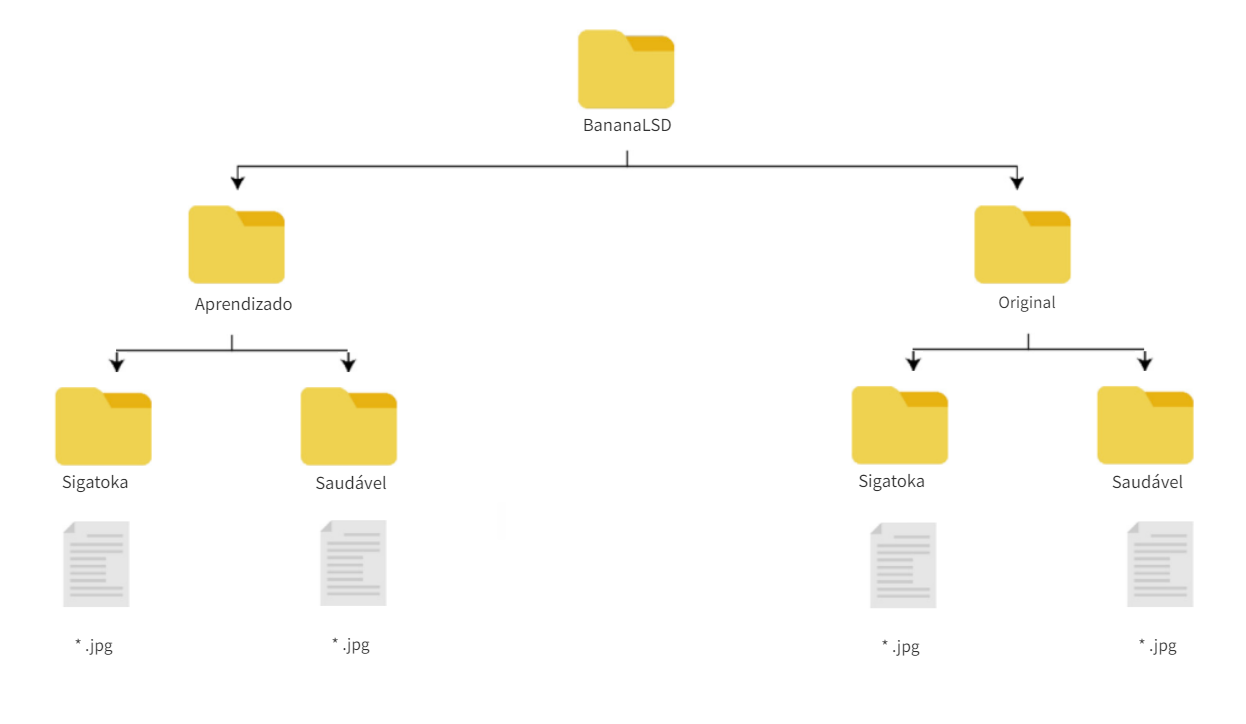
\includegraphics[width=11cm]{figuras/Pastas.png}\\
	\autoria{Autoria Própria (2024)}
	\label{fig:Pastas}
\end{figure}

\section{Implementação do Aprendizado de Máquina}
Para a tarefa de classificar imagens de folhas de bananeira, foi escolhido utilizar \ac{RNC}, já que são especialmente eficazes para reconhecimento de padrões em imagens. Isso acontece porque as \ac{RNC}s conseguem capturar características espaciais e hierárquicas da estrutura geral das imagens.

A decisão de usar \ac{RNC}s também se justifica pelos resultados positivos que elas já demonstraram em estudos anteriores sobre a detecção de doenças em plantas. Além disso, elas são capazes de lidar bem com grandes volumes de dados e com a complexidade das imagens, o que é exatamente necessário para o projeto.

Na Figura \ref{Fig:RezendeMet}, apresenta-se um diagrama detalhado que ilustra cada etapa do processo metodológico. Esse diagrama ajuda a entender a estrutura e organização do trabalho, de modo a facilitar a apresentação do objetivo de desenvolver uma classificação eficaz.

\begin{figure}[!h]
	\centering
	\caption{Metodologia para a classificação de imagens de doenças em plantas.}
	%\vskip 5mm
	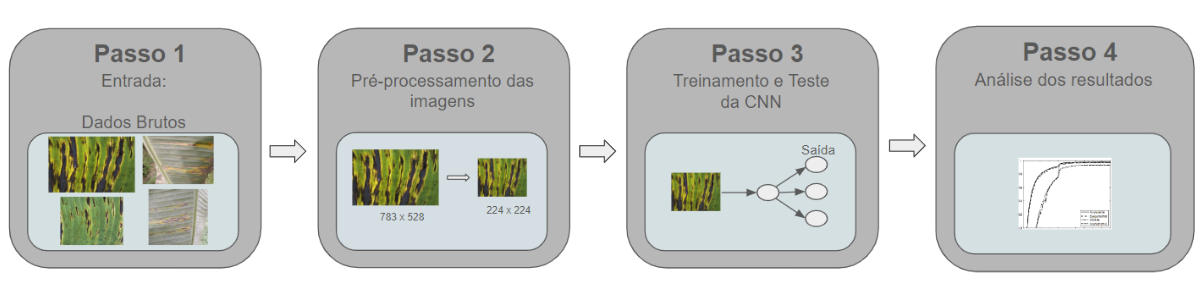
\includegraphics[width=15cm]{figuras/RezendeMetodos.png}\\
	\autoria{Autoria Própria (2024)}
	\label{Fig:RezendeMet}
\end{figure}

Primeiro, começamos selecionando a base de dados que será usado como entrada para o algoritmo. Em seguida, passamos para o pré-processamento das imagens, uma etapa importante em que ajustamos todas as imagens com as técnicas apresentadas, adaptamos todas para terem o mesmo tamanho e também removemos aquelas que poderiam atrapalhar a análise.

Com todos os dados padronizados, inicia-se a fase de treinamento e teste das RNCs, momento em que as redes começam a extrair as características mais relevantes das imagens. Por fim, realiza-se a análise de desempenho dos resultados, avaliando-se o comportamento das RNCs. Caso alguma anomalia seja detectada, ajustam-se os parâmetros necessários e reinicia-se o treinamento da rede.

\subsection{Escolha do Modelo de \ac{RNC}}
No início, apesar de as Redes Neurais Convolucionais serem amplamente conhecidas nas comunidades de visão computacional e aprendizado de máquina, elas não se tornaram imediatamente predominantes na área. Esse cenário mudou radicalmente em 2012, quando a AlexNet, uma \ac{RNC} com 8 camadas, conquistou o Desafio de Reconhecimento Visual em Grande Escala ImageNet com uma ampla vantagem~\cite{Art4}. Desde então, essa rede demonstrou pela primeira vez que o aprendizado profundo poderia superar os métodos projetados manualmente.

Conforme ilustrado na Figura~\ref{Fig:ArquitAlexnet}, a arquitetura da AlexNet é composta por cinco camadas convolucionais, seguidas por três camadas totalmente conectadas. Nas duas primeiras camadas e na quinta, cada uma é acompanhada por uma camada de max-pooling. Já a terceira e a quarta camadas são conectadas diretamente, sem nenhuma outra estrutura intermediária. A última camada da rede é utilizado a função de ativação softmax com 1000 unidades, correspondendo a cada rótulo possível.

\begin{figure}[!h]
	\centering
	\caption{Arquitetura Simplificada da Alexnet.}
	%\vskip 5mm
	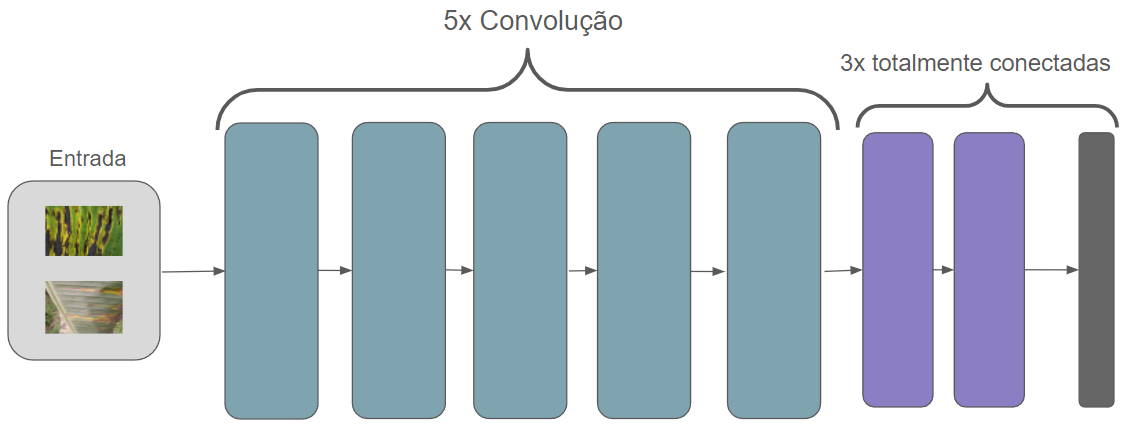
\includegraphics[width=15cm]{figuras/ArquitAlexnet.png}\\
	\autoria{Autoria Própria (2024)}
	\label{Fig:ArquitAlexnet}
\end{figure}

A arquitetura AlexNet utiliza funções de ativação \ac{ReLU} nas primeiras sete camadas da rede neural. Essas funções de ativação são conhecidas por acelerar o processo de treinamento ao introduzir não-linearidades, permitindo que a rede aprenda a representar funções complexas de forma mais eficiente.

O \textit{overfitting} ocorre quando a rede aprende a memorizar padrões específicos dos dados de treino, apresentando bom desempenho apenas nesses casos específicos, mas falhando ao generalizar para novos dados. Uma das principais estratégias utilizadas na AlexNet para combater o \textit{overfitting} é o \textit{dropout}. Essa técnica funciona ao desligar aleatoriamente neurônios durante o treinamento, com uma probabilidade de 50\% \cite{braga2021avaliacao}. Esse desligamento aleatório dos neurônios altera efetivamente a arquitetura da rede para cada entrada, ajudando a evitar que a rede se torne excessivamente dependente de qualquer neurônio ou conjunto de neurônios específicos.

\section{Metodologia de Avaliação dos Resultados}
A avaliação do desempenho de uma rede neural artificial projetada é uma etapa crucial para assegurar a qualidade dos sistemas de classificação. Existem diversas abordagens para verificar a eficácia do classificador desenvolvido.

As principais métricas aplicadas na análise de desempenho do sistema projetado foram a \ac{MC} e a  \ac{Ac}. A Figura~\ref{FIG:matriz} ilustra um exemplo de \ac{MC}, onde as classificações corretas aparecem na diagonal principal, enquanto as outras posições da matriz indicam erros de classificação. Somando-se os valores de cada linha $i$ que não estão na diagonal principal, obtêm-se os \ac{FP} da classe $i$, que representam as vezes em que o modelo previu incorretamente a classe $i$. Por outro lado, ao somar os elementos de cada coluna $j$, excluindo-se as células da diagonal principal, obtêm-se os \ac{FN} da classe $j$, que indicam objetos pertencentes à classe $i$ classificados erroneamente como de outras classes. Os \ac{TN} são determinados somando os elementos restantes, após a exclusão da linha e coluna correspondentes à classe $i$ \cite{silva2022sistema}.

\begin{figure}[!h]
	\centering
	\caption{Matriz de confusão.}
	%\vskip 5mm
	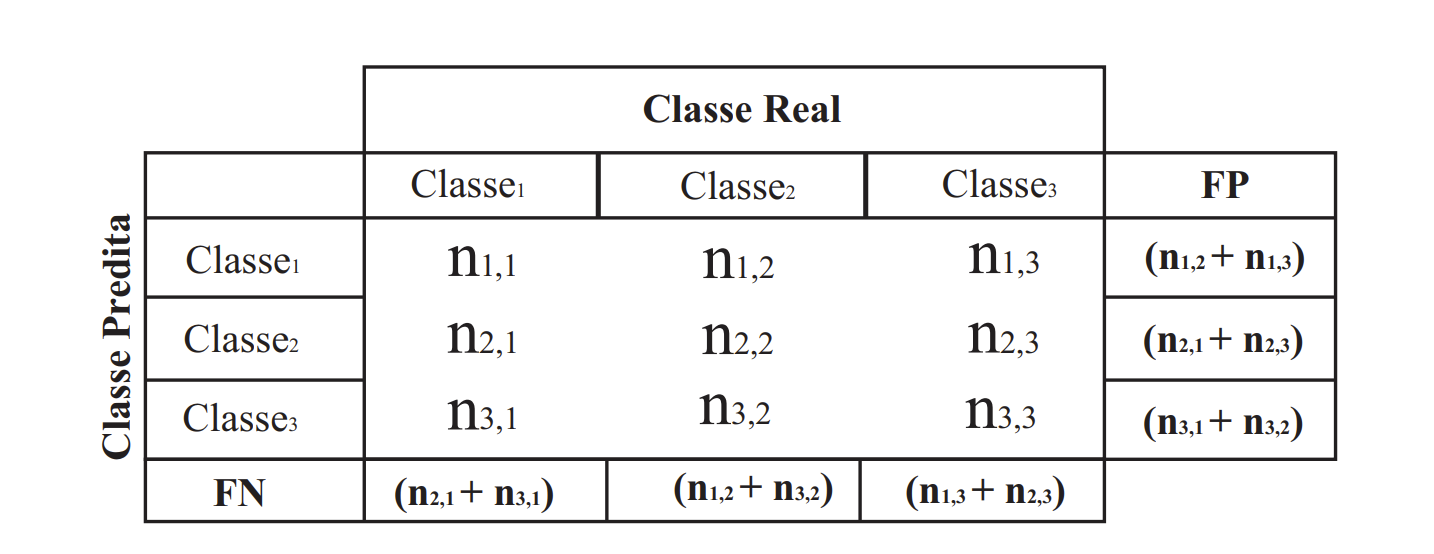
\includegraphics[width=13cm]{figuras/confusion1.png}\\
	\autoria{\cite{silva2022sistema}}
	\label{FIG:matriz}
\end{figure}

Diversas métricas de desempenho podem ser derivadas da matriz de confusão para avaliar o classificador desenvolvido. A \ac{Ac} é uma dessas métricas e representa a performance geral do modelo, indicando a proporção de acertos em relação ao número total de classificações realizadas (Equação~\ref{eq:1}). Já o erro de classificação ($Cf$) pode ser calculada pela Equação~\ref{eq:2}, expressando a relação entre as classificações incorretas e o total de classificações \cite{silva2022sistema}.   

\begin{equation}
\label{eq:1}
Ac = \frac{\sum_{i=1}^{m} n_{i,j}}{\sum_{i=1}^{m}\sum_{j=1}^{m}n_{i,j}}
\end{equation}

\begin{equation}
\label{eq:2}
Cf = 1 - Ac
\end{equation}


\section{Especificação de Máquina e Software}
As especificações da máquina utilizada incluem uma CPU Ryzen 7 5700X de 8 núcleos e 16 threads, com frequência de 3.2 GHz, e uma memória RAM de 16 GB. Para o treinamento, foi utilizada uma GPU AMD Radeon RX 580 com interface de memória de 8 GB GDDR5 de 256 bits.

O ambiente de desenvolvimento utilizado neste trabalho incluiu o Anaconda, que facilitou a gestão de pacotes e ambientes, o Jupyter Notebook para o desenvolvimento e execução interativos dos códigos, e a biblioteca PyTorch, configurada com suporte a GPUs para acelerar o treinamento de modelos.

% \begin{equation}
% Ac = \frac{\sum_{i=1}^{m} n_{i,j}}{\sum_{i=1}^{m} \sum_{j=1}^{m} n_{i,j}}
% \end{equation}


% O modelo AlexNet foi treinado ao longo de 100 épocas, com um batch size de 120 e utilizando a função de perda cross entropy. O uso do otimizador Adam com uma taxa de aprendizado inicial de 0.0001, ao invés do SGD proposto no artigo original, foi crucial para garantir a convergência do treinamento. Observou-se que o uso do SGD, conforme os parâmetros originais, não produziu resultados satisfatórios, indicando que os hiperparâmetros requerem ajustes específicos para diferentes datasets e contextos.

% Durante o treinamento, a acurácia foi monitorada em intervalos regulares. A implementação logou os valores de perda e acurácia no TensorBoard, permitindo uma análise visual da performance do modelo. A acurácia apresentou melhorias consistentes ao longo das épocas, confirmando a capacidade da AlexNet de aprender as características das imagens e diferenciá-las entre as duas classes. No entanto, a precisão exata do modelo ao final das 100 épocas não foi explicitada no código, mas pode ser inferida a partir dos logs gerados.

% Uma característica importante desta implementação foi a análise dos gradientes e dos parâmetros do modelo em pontos regulares durante o treinamento. Isso permitiu a identificação de possíveis problemas, como gradientes desvanecendo ou explodindo, e ajudou a assegurar que o treinamento estava progredindo corretamente. A análise das distribuições de gradientes e pesos no TensorBoard contribuiu para uma melhor compreensão do comportamento do modelo durante o treinamento.

% O uso de um agendador de taxa de aprendizado (StepLR) que reduziu a taxa de aprendizado em um fator de 10 a cada 30 épocas foi eficaz em refinar o treinamento do modelo. Este método ajudou a evitar que o modelo ficasse preso em mínimos locais e melhorou a capacidade do AlexNet de generalizar, ao permitir ajustes mais finos na fase final do treinamento.


% A função de visualização de algumas imagens do conjunto de dados permitiu verificar a correta aplicação das transformações e a adequação das imagens para o treinamento. Esse passo é importante para garantir que o pipeline de dados está funcionando corretamente e que as imagens estão sendo processadas conforme esperado.

% O salvamento regular de checkpoints ao final de cada época permitiu preservar o estado do modelo, possibilitando retomar o treinamento de um ponto intermediário, se necessário. Isso é essencial em treinamentos longos para mitigar a perda de progresso devido a falhas ou interrupções inesperadas.

% Em resumo, a implementação do AlexNet e os resultados obtidos demonstram a eficácia da rede para tarefas de classificação de imagens, mesmo em datasets menores e com menos classes, como o utilizado neste experimento. O uso de ferramentas como o TensorBoard para monitoramento contínuo e ajustes no treinamento se mostrou vital para alcançar uma boa performance. Contudo, é importante destacar que o ajuste fino dos hiperparâmetros, como a escolha do otimizador, desempenha um papel crucial para a adaptação do modelo a diferentes contextos e datasets.

% A exploração futura pode incluir testes com diferentes taxas de aprendizado, otimizadores, e o uso de técnicas de regularização mais avançadas para melhorar ainda mais a generalização do modelo.

% \newpage



% \subsection{Módulo sensor}

% Para a aquisição de dados do ambiente foram utilizados sensores de temperatura, umidade do solo e umidade relativa do ar. Como mencionado no capítulo anterior, o sensor de temperatura escolhido para o projeto foi o DHT-22, que possui características descritas na Tabela \ref{tab:my-table4}, pois suas especificações de precisão, estabilidade, durabilidade e condições operacionais se encaixam nos requisitos do projeto. O seu protocolo de 1- Barramento permite a conexão de múltiplos sensores em uma única entrada do microcontrolador, isso permite com que sejam utilizados vários sensores em pontos distintos da estufa, obtendo valor mais abrangente da temperatura ambiente sem a necessidade de ocupar mais portas lógicas do microcontrolador.


% \begin{table}[!h]
% \centering
% \caption{Características de temperatura do sensor DHT-22.
% }
% \label{tab:my-table4}
% \begin{tabular}{c|c}
% \hline
% \textbf{Características}    & \textbf{Valor}                                                                                                               \\ \hline
% Alimentação                 & 3,0V a 6,0V                                                                                                                  \\ \hline
% Temperatura de operação     & -55°C a 125°C                                                                                                                \\ \hline
% Precisão entre -10°C a 85°C & 0,5°C                                                                                                                        \\ \hline
% Pinagem                     & \begin{tabular}[c]{@{}c@{}}Vermelho: Tensão de corrente contínua (VCC)\\ Amarelo: Dados\\ Preto: Referência/GND\end{tabular} \\ \hline
% Comprimento do cabo         & 1 m                                                                                                                          \\ \hline
% Protocolo                   & 1- Barramento                                                                                                                \\ \hline
% \end{tabular}
% \\
% \autoria{\cite{gomes2017calibraccao}}
% \end{table}

% Para mensurar a umidade relativa do ar foi utilizado o sensor DHT-22, suas características de funcionamento são expostas na Tabela \ref{tab:my-table5}, esse sensor possui a capacidade de medir tanto a umidade relativa do ar, quanto a temperatura ambiente, tem como vantagem o baixo custo e a grande quantidade de trabalhos desenvolvidos com ele na literatura.

% \begin{table}[!h]
% \centering
% \caption{Características de umidade do ar do sensor DHT-22.
% }
% \label{tab:my-table5}
% \begin{tabular}{c|c}
% \hline
% \textbf{Características} & \textbf{Valor}                                                                                              \\ \hline
% Alimentação              & 3,0V a 6,0V                                                                                                   \\ \hline
% Umidade de operação      & 0 a 100\%                                                                                                   \\ \hline
% Precisão                 & 2\%                                                                                                         \\ \hline
% Pinagem                  & \begin{tabular}[c]{@{}c@{}}Pino 1: Tensão de corrente contínua (VCC)\\ Pino 2: Dados\\ Pino 3: Referência/GND\end{tabular} \\ \hline
% Sinal de saída           & Sinal digital via barramento único                                                                          \\ \hline
% \end{tabular}
% \\
% \autoria{\cite{gomes2017calibraccao}}
% \end{table}

% Foi desenvolvido um módulo sensor contendo os componentes necessários para o funcionamento do DHT-22, Sendo composto por um resistor de 4,7K que foi ligado entre o pino de alimentação positiva e o pino de dados, sendo utilizado para garantir que o sinal ficará em um nível lógico conhecido quando o pino não estiver enviando sinal, também foi utilizado um capacitor de 100nF entre os pinos de alimentação positiva e negativa, para filtrar ruídos de alta frequência que podem distorcer o sinal de dados, as ligações foram realizadas de acordo com a Figura \ref{fig:LDHT22}. 

% \begin{figure}[!h]
% 	\centering
% 	\caption{Esquema de ligação do módulo DHT22}
% 	%\vskip 5mm
% 	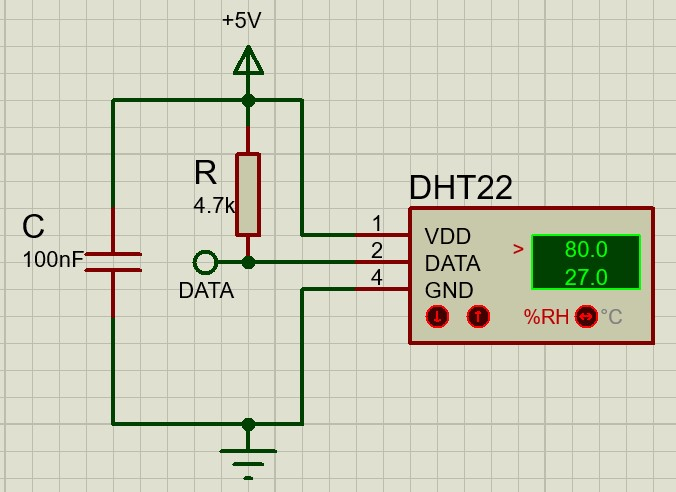
\includegraphics[width=7cm]{figuras/image.png}\\
% 	\autoria{Autoria própria}
% 	\label{fig:LDHT22}
% \end{figure}

% Para garantir uma boa conexão entre os componentes, o módulo foi desenvolvido em uma placa de circuito impresso e seus componentes foram isolados com o uso de um tubo termo retrátil, foram utilizados fios de alumínio cobreado para prolongar os pinos do módulo e aumentar a distancia em que ele pode ficar do módulo de condicionamento de sinais, o protótipo é apresentado na Figura \ref{fig:MDHT22}.


% \begin{figure}[!h]
% 	\centering
% 	\caption{Módulo DHT22}
% 	%\vskip 5mm
% 	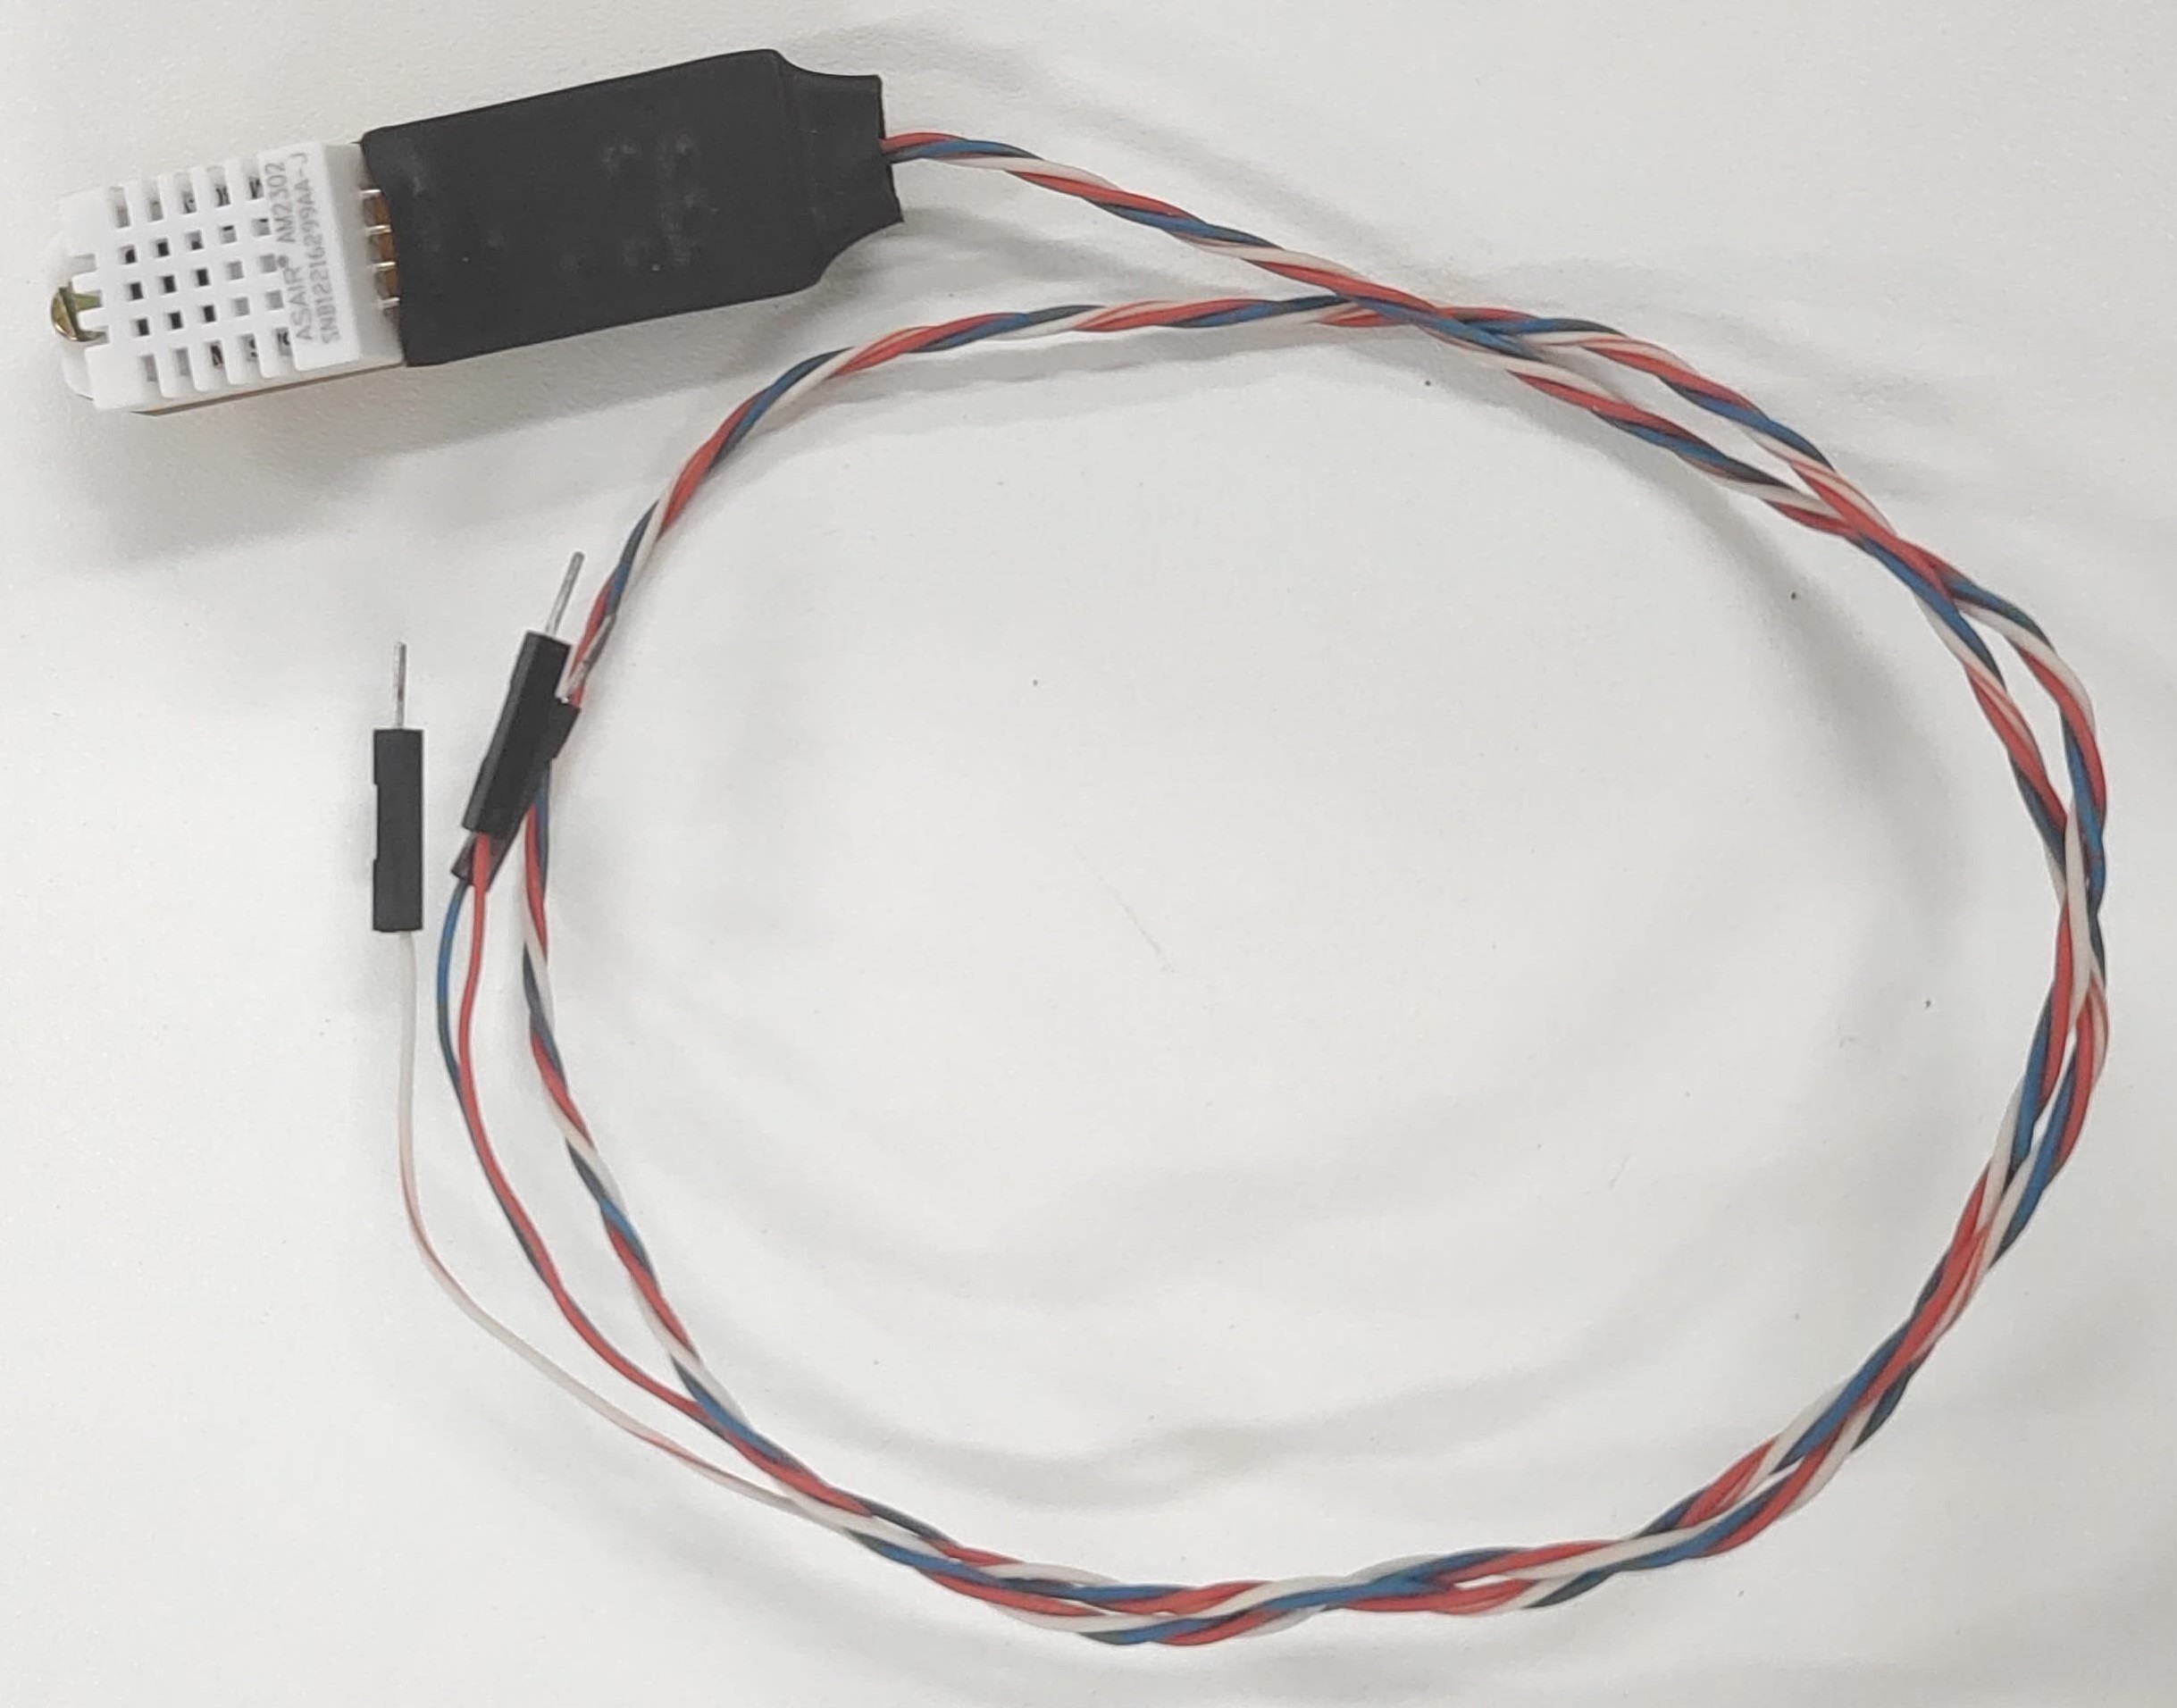
\includegraphics[width=6cm]{figuras/MEUDHT22.jpeg}\\
% 	\autoria{Autoria própria}
% 	\label{fig:MDHT22}
% \end{figure}

% O sensor de umidade do solo HD-38 possui encapsulamento de metal, tornando resistente a corrosões causadas pelo contato contínuo com o solo, como apresentado na Tabela \ref{tab:my-table6}, suas características o tornam ideal para o projeto.


% \begin{table}[!h]
% \centering
% \caption{Características do sensor HD-38.
% }
% \label{tab:my-table6}
% \begin{tabular}{c|c}
% \hline
% \textbf{Características} & \textbf{Valor}                                                                                              \\ \hline
% Alimentação              & 3,3V a 12,0V                                                                                                \\ \hline
% Umidade de operação      & 0 a 100\%                                                                                                   \\ \hline
% Precisão                 & 1\%                                                                                                         \\ \hline
% Pinagem                  & \begin{tabular}[c]{@{}c@{}}Pino 1: Tensão de corrente contínua (VCC)\\Pino 2: Dados\\Pino 3: Referência/GND\end{tabular} \\ \hline
% Comprimento do cabo      & 1 m                                                                                                         \\ \hline
% \end{tabular}
% \\
% \autoria{\cite{gomes2017calibraccao}}
% \end{table}

% Os sensores foram posicionados em pontos estratégicos na estufa, visando a captura de dados de maneira homogênea. Cada módulo de sensores é composto por um sensor DHT-22 e um HD-38. O módulo foi conectado fisicamente ao circuito de condicionamento de sinais, que fornece a alimentação dos sensores.  

% \subsection{Módulo atuador}

% O módulo de atuadores é conectado fisicamente ao circuito de condicionamento de sinais, que é responsável por transmitir os comandos a serem executados pelos atuadores, além de captar o estado atual de cada atuador. A composição do módulo depende das características do local onde é aplicado, podendo conter relés para acionamento de cargas como motores, ventiladores e bombas, além de válvulas solenoides para controlar o fluxo de água. Para os testes realizados, foi utilizado um módulo relé de quatro canais, como visto na Figura \ref{fig:RELE}.

% \begin{figure}[!h]
% 	\centering
% 	\caption{Módulo relé}
% 	%\vskip 5mm
% 	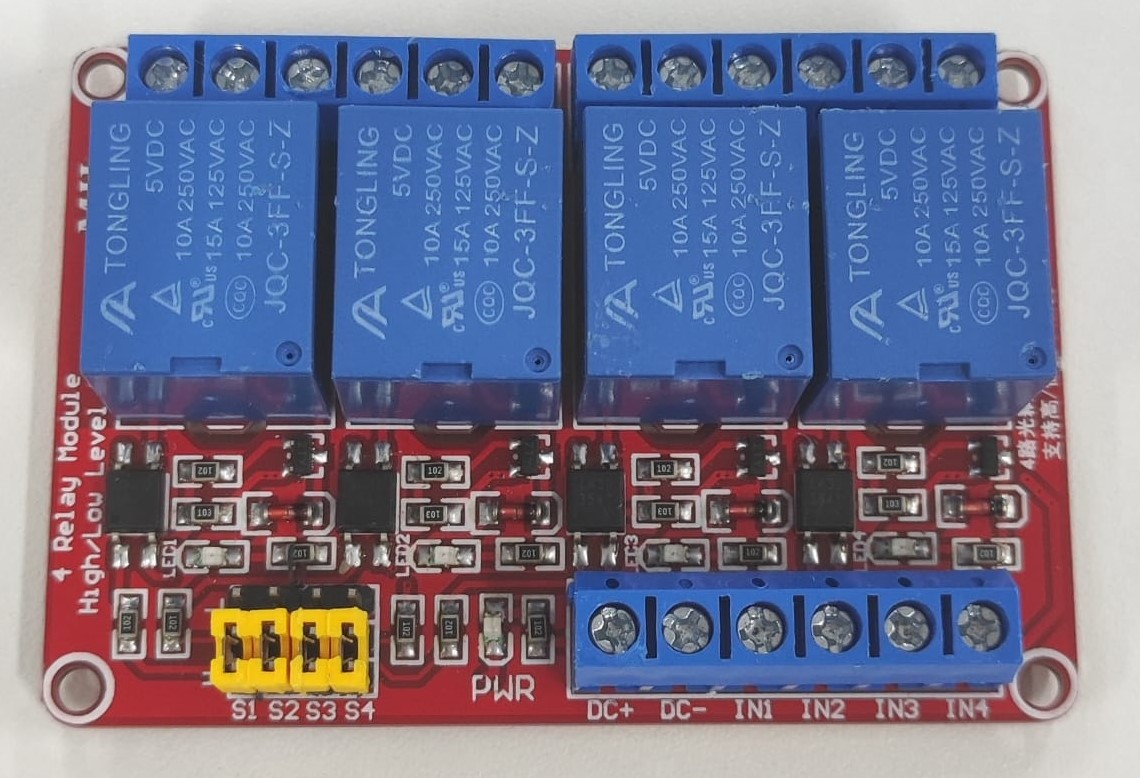
\includegraphics[width=8cm]{figuras/RELE.jpeg}\\
% 	\autoria{Autoria própria}
% 	\label{fig:RELE}
% \end{figure}

% \subsection{Circuito de condicionamento de sinais}

% O circuito de condicionamento de sinais tem função muito importante no projeto, ele é responsável por captar os dados dos sensores, condiciona-los e processa-los. Esta etapa realiza o controle dos atuadores, de maneira independente do módulo central, esse controle ocorre independente de conexão com internet ou \ac{Wi-Fi}, implicando maior confiabilidade ao sistema, pois perdas de conexão não afetam as funções de aquisição de dados dos sensores e controle dos atuadores.

% Este circuito é composto por microcontrolador PIC18F4550 e circuito eletrônico necessário para o seu funcionamento, que é fornecido pela placa \textit{microStart}, que conta com oscilador externo de 20 MHz, entrada USB tipo B e conector P4 para alimentação de 6V a 15V contínuos, a placa utilizada é vista na Figura \ref{fig:PICP}. 

% \begin{figure}[!h]
% 	\centering
% 	\caption{Placa PIC}
% 	%\vskip 5mm
% 	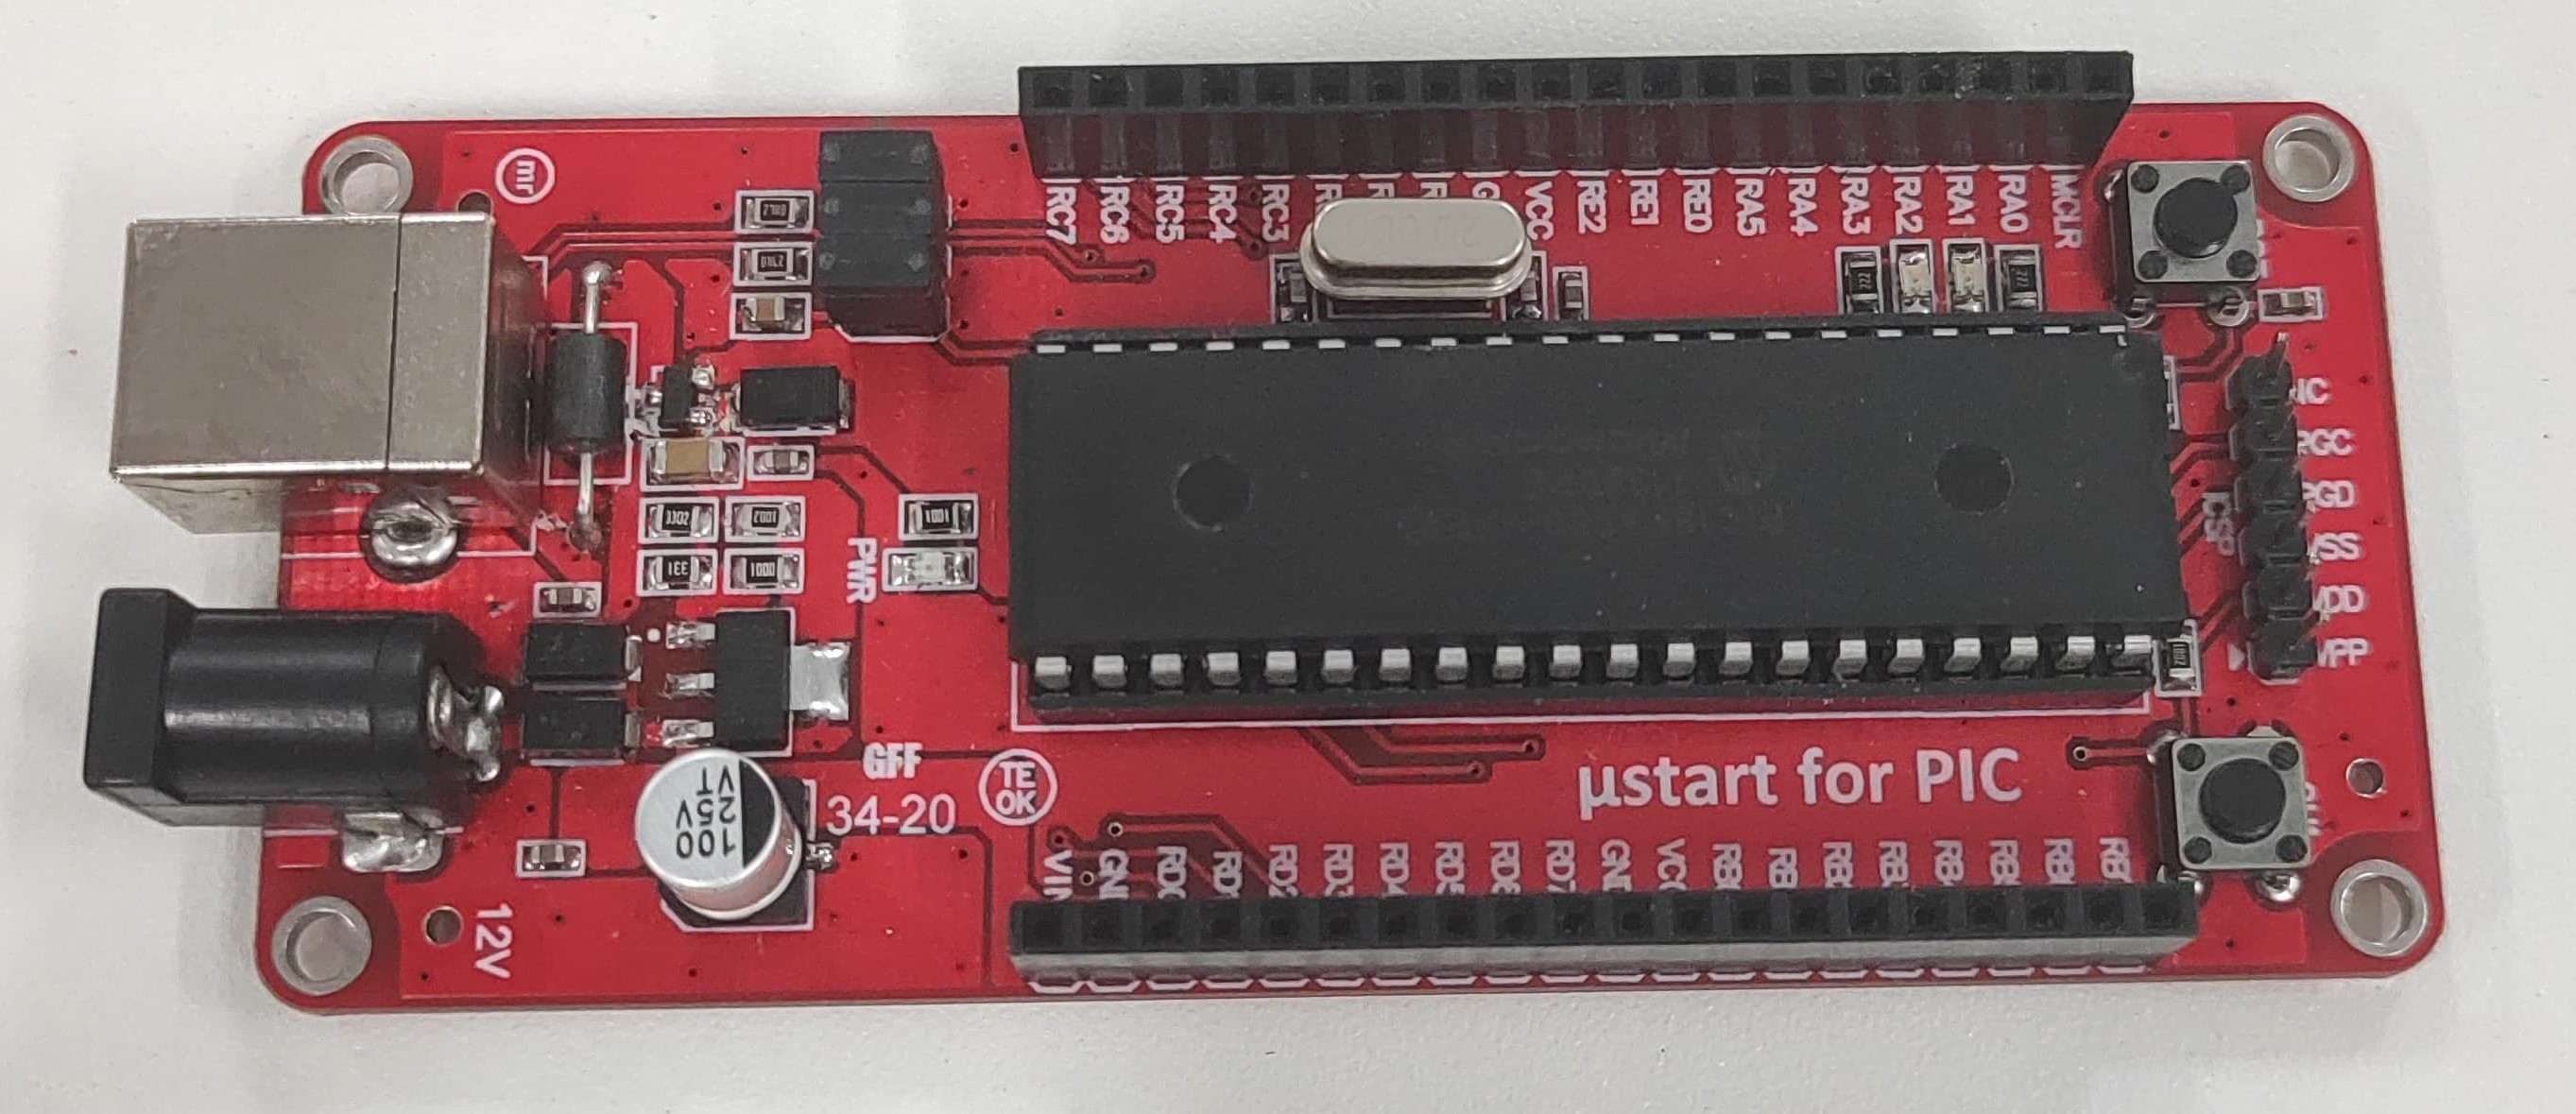
\includegraphics[width=10cm]{figuras/PLACAPIC.jpeg}\\
% 	\autoria{Autoria própria}
% 	\label{fig:PICP}
% \end{figure}

% Conta também com circuito de comunicação via radiofrequência para se conectar com o módulo central, além de fonte de alimentação composta por módulos fotovoltaicos e baterias, caso a estufa esteja em uma localidade que não tenha disponibilidade de energia elétrica, na Figura \ref{fig:ligac} é apresentado o esquema de ligação entre os componentes do circuito.

% \begin{figure}[!h]
% 	\centering
% 	\caption{Esquema de ligação do módulo de condicionamento de sinais}
% 	%\vskip 5mm
% 	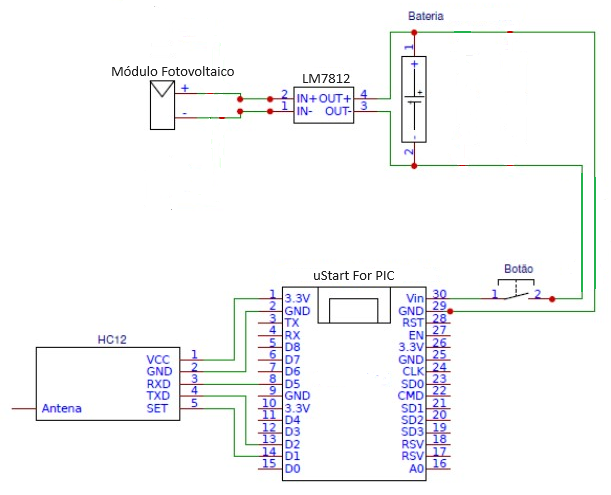
\includegraphics[width=10cm]{figuras/esquemaligac.png}\\
% 	\autoria{Autoria própria}
% 	\label{fig:ligac}
% \end{figure}

% Para garantir uma alimentação mais estável para o sistema, foi desenvolvido um módulo regulador de tensão, composto por um circuito integrado LM7812, que tem como função regular tensões entre 21V até 13V em uma tensão de 12V contínuos, foi inserido um capacitor de 100nF paralelo à saída do módulo para filtrar ruídos de alta frequência, o esquema de ligação do regulador é apresentado na Figura \ref{fig:reg}. Dessa forma, o sistema pode ser alimentado pelos módulos fotovoltaicos e bateria, como também por meio de uma fonte externa, ligada à tomada, como as usadas para carregar notebook.

% \begin{figure}[!h]
% 	\centering
% 	\caption{Esquema de ligação do regulador de tensão}
% 	%\vskip 5mm
% 	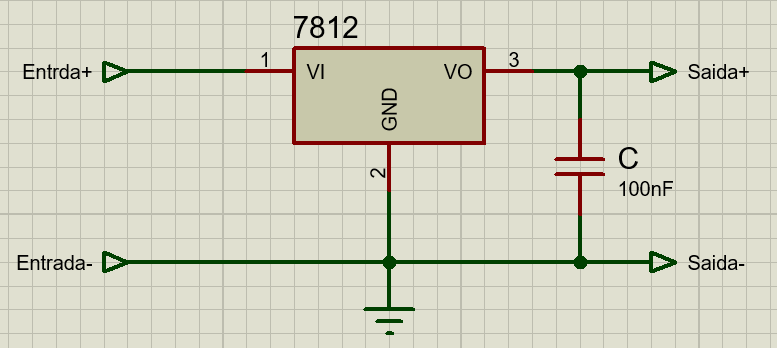
\includegraphics[width=10cm]{figuras/regulador.png}\\
% 	\autoria{Autoria própria}
% 	\label{fig:reg}
% \end{figure}

% Após a montagem física do circuito contendo módulo fotovoltaico de 15V, bateria de 12V, placa com PIC e os componentes que compõem o circuito de condicionamento de sinais, o protótipo é exibido na Figura \ref{fig:cond}.

% \begin{figure}[!h]
% 	\centering
% 	\caption{Módulo de condicionamento de sinais}
% 	%\vskip 5mm
% 	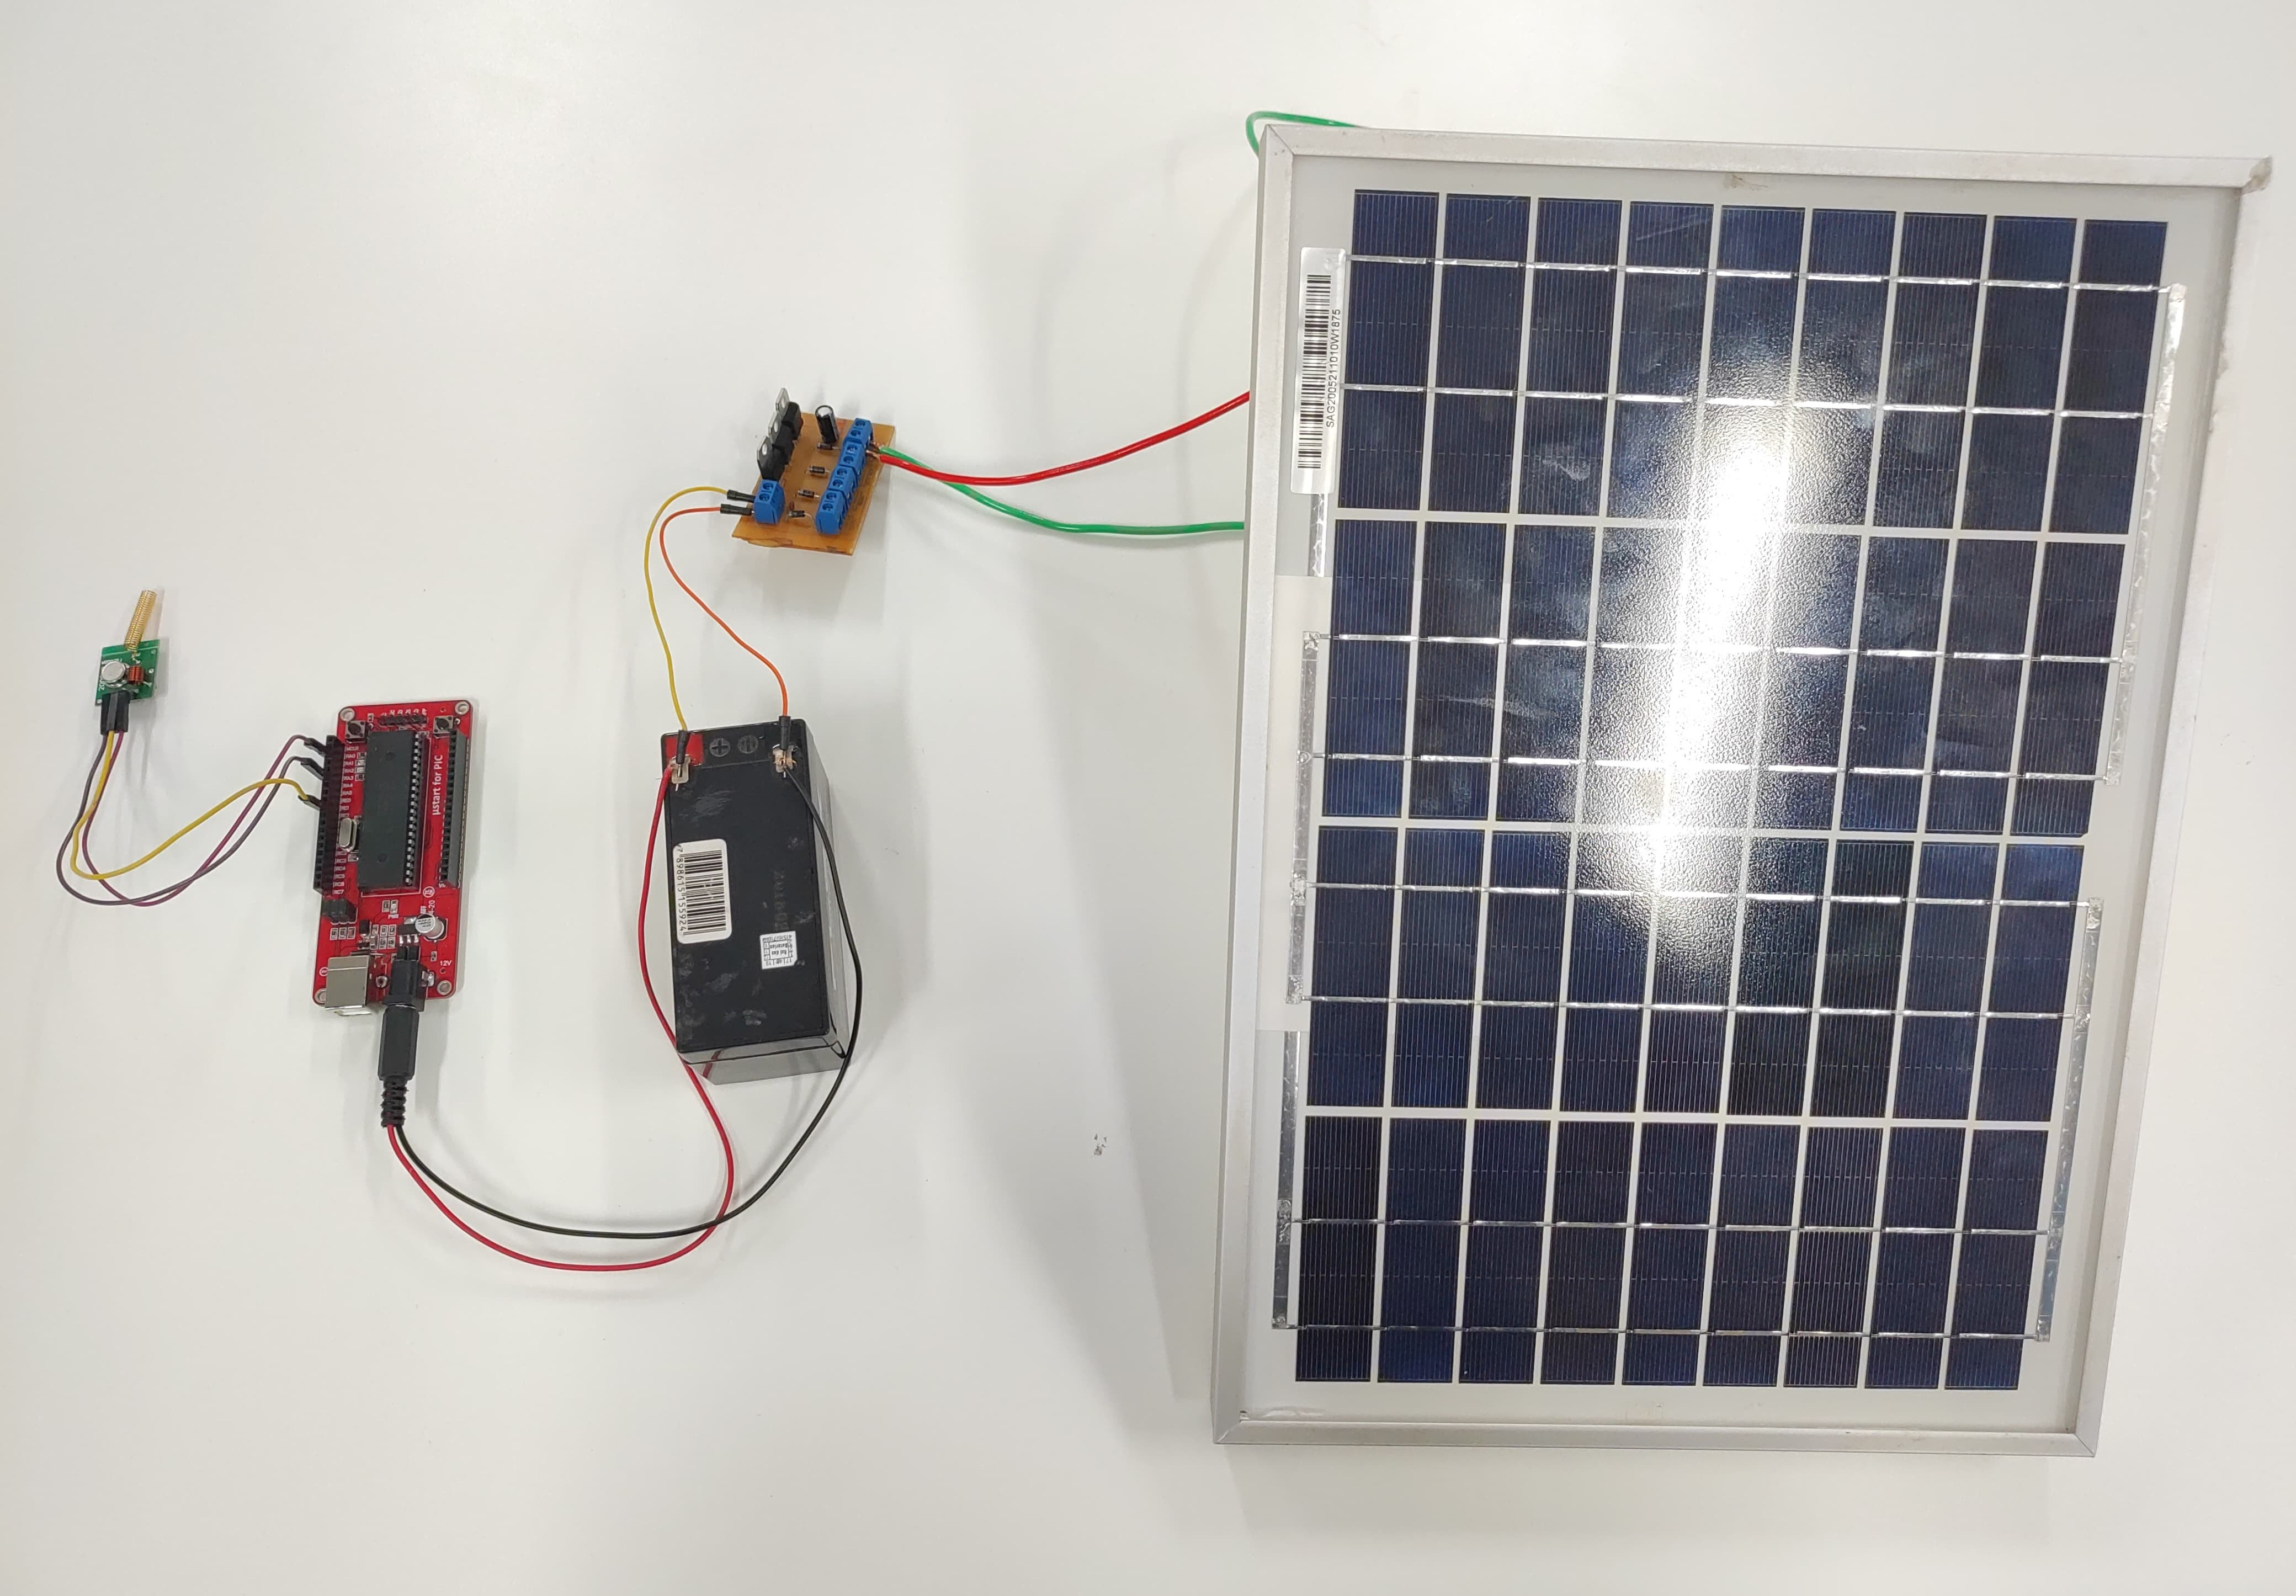
\includegraphics[width=10cm]{figuras/coisasmontadas.jpeg}\\
% 	\autoria{Autoria própria}
% 	\label{fig:cond}
% \end{figure}

% \subsection{Envio de dados}

% O envio de dados ocorre de diferentes maneiras entre os módulos. Entre os sensores, atuadores, interface Humano/Máquina física e circuito de condicionamento de sinais, os dados são enviados utilizando conexões físicas, por meio de cabos. A comunicação entre o circuito de condicionamento de sinais e o módulo central é realizada por radiofrequência utilizando dois módulos RF HC-12, que permitem uma conexão de até 6,5km entre os módulos. A troca de informações entre o módulo central e a interface Humano/Máquina virtual ocorre com o protocolo \ac{MQTT}.

% O protocolo MQTT foi implementado no ESP32, tendo esse a função de publicador principal, enviando os dados para o \textit{broker}. Foi utilizado um \textit{broker} gratuito chamado hivemq.com, de domínio público e utilizado para desenvolvimento de protótipos. Foi criado o tópico estufaautomatica/\textit{publisher}, onde serão publicados os dados enviados pelo ESP32 e os inscritos no tópico poderão receber esses dados. Dessa forma, foi inscrito no tópico a interface gráfica \textit{web}, que pode ser acessada por dispositivo conectado à internet.

% \subsection{Interface Humano/Máquina}

% A apresentação dos dados dos sensores e estados dos atuadores é realizada por meio de duas interfaces, sendo uma de maneira física conectada ao circuito de condicionamento de sinais, permitindo que funcione independentemente da conexão com o módulo central ou internet. A placa contem um visor onde são apresentados os dados dos sensores, LED's que indicam o estado dos atuadores, a existência de conexão com o módulo central e a indicação de placa energizada, e botões onde podem ser realizados teste de funcionamento dos atuadores e também a configuração e escolha do tipo de plantação a ser cultivada. Na Tabela \ref{tab:led} são apresentados as cores dos LED's e seus significados.

% \begin{table}[!h]
% \centering
% \caption{Descrição das cores}
% \label{tab:led}
% \begin{tabular}{c|c}
% \hline
% Cor do LED & Indicação \\ \hline
% Vermelho & Sistema energizado \\ \hline
% Azul & Comunicação com a IHM virtual \\ \hline
% Verde & Irrigação ativada \\ \hline
% Amarelo & Ventilação ativada \\ \hline
% \end{tabular}
% \\
% \autoria{Autoria própria}
% \end{table}

% A configuração do sistema ocorre de maneira simplificada, sedo acessível para pessoas com pouca afinidade com tecnologia. Para realizar a escolha da plantação, basta apertar o botão \textit{ENTER} a qualquer momento e entrar no menu de opções, em seguida pode-se navegar através dos botões para cima e para baixo, representados por setas, ao encontrar a opção desejada, aperta-se novamente o botão \textit{ENTER} e a escolha foi concluída.


% A interface foi desenvolvida em placa de circuito impresso para fornecer maior confiabilidade e resistência em suas conexões, além do posicionamento dos componentes oferecer simplicidade ao usuário, como pode ser visto na Figura \ref{fig:IHMP}.

% \begin{figure}[!h]
% 	\centering
% 	\caption{IHM física}
% 	%\vskip 5mm
% 	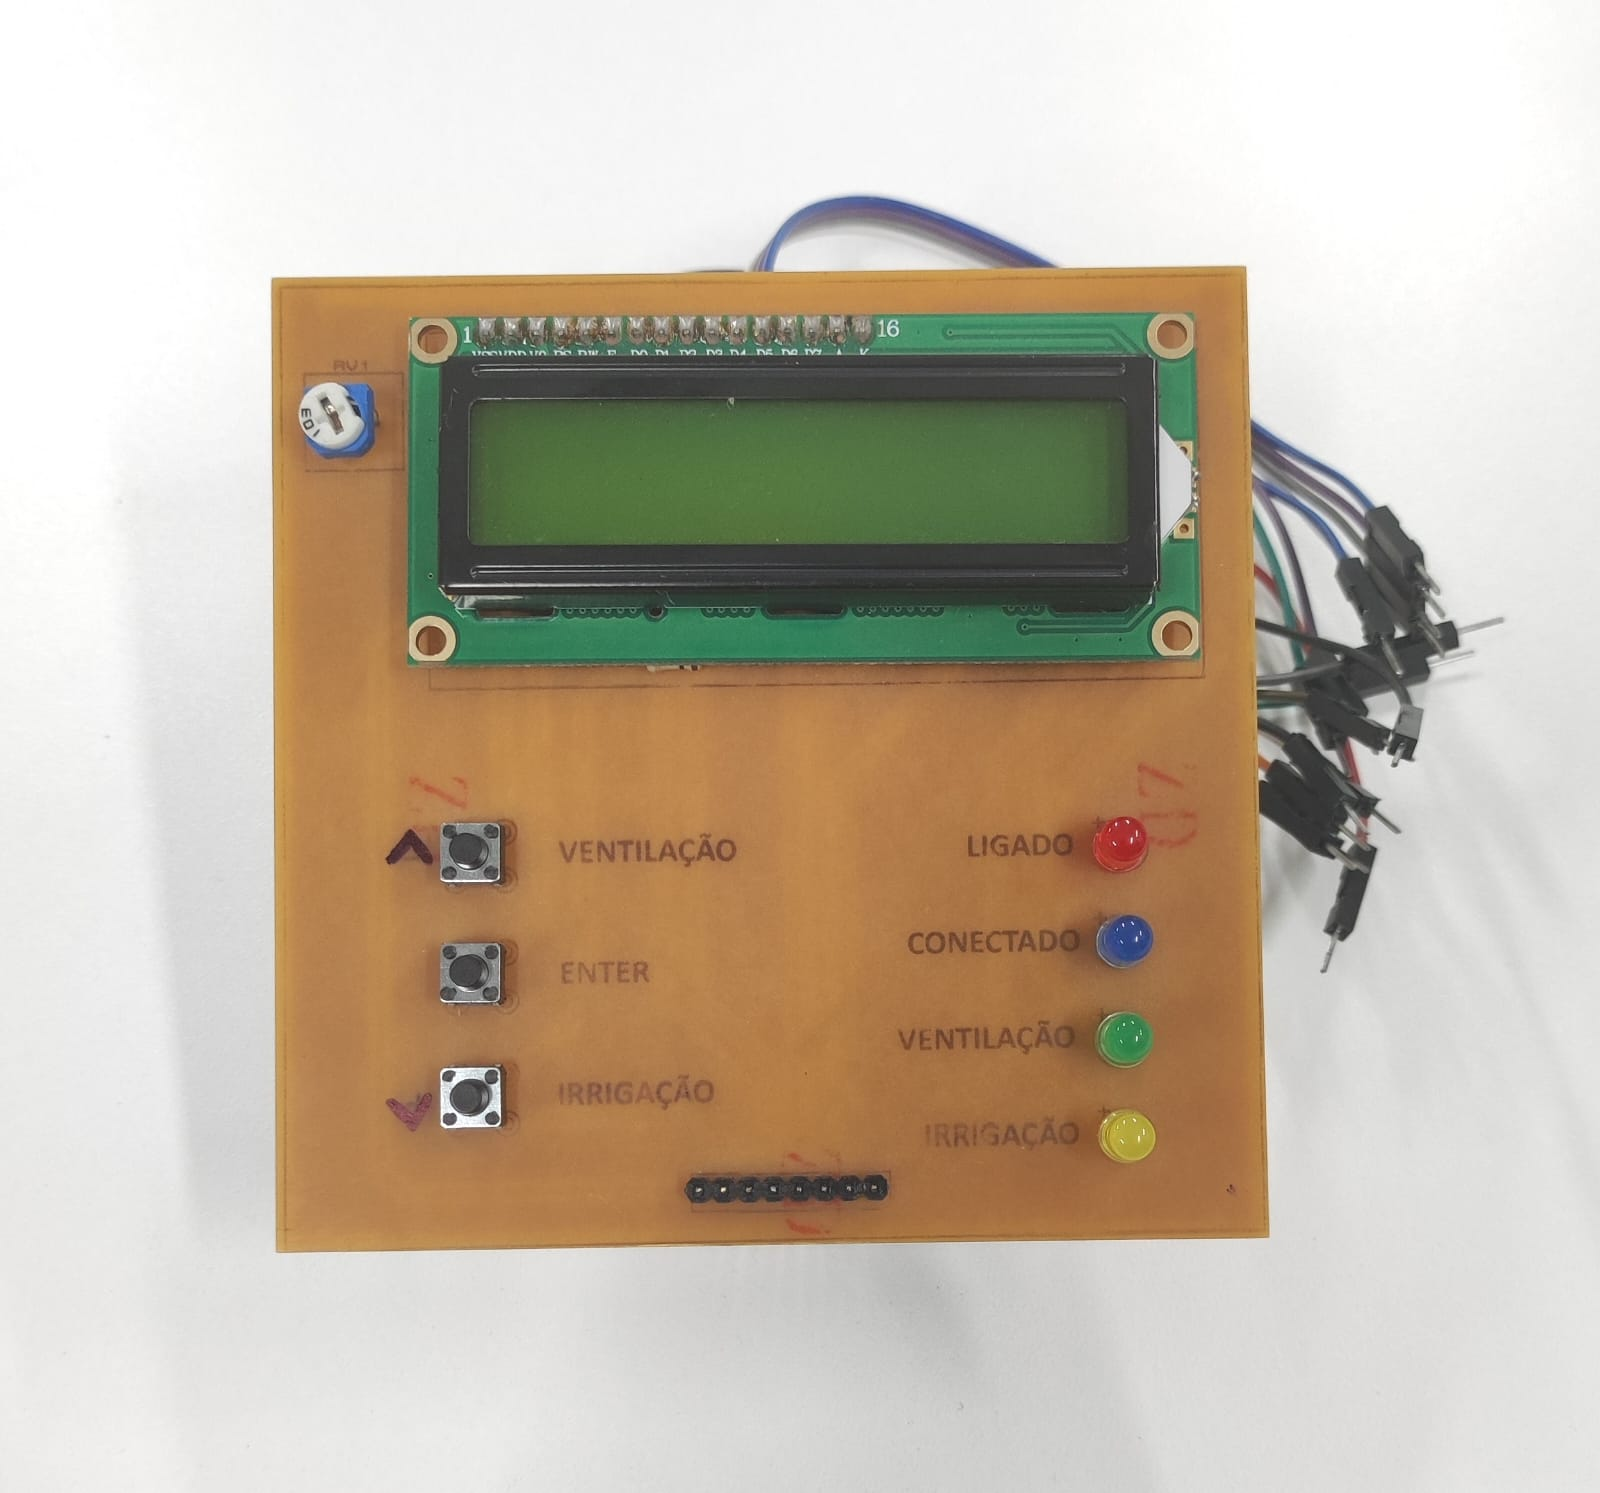
\includegraphics[width=10cm]{figuras/MINHAIHM.jpeg}\\
% 	\autoria{Autoria própria}
% 	\label{fig:IHMP}
% \end{figure}

% A interface gráfica que pode ser acessada por meio de computador ou celulares conectados à internet. Foi desenvolvido um aplicativo simples, usando a plataforma \textit{MIT App Inventor 2}, que fornece suporte para aplicações com protocolo MQTT. Essa plataforma permite o desenvolvimento de aplicativos usando programação em blocos simplificados, conforme Figura \ref{fig:progbloco}.

% \begin{figure}[!h]
% 	\centering
% 	\caption{Programação em blocos do aplicativo}
% 	%\vskip 5mm
% 	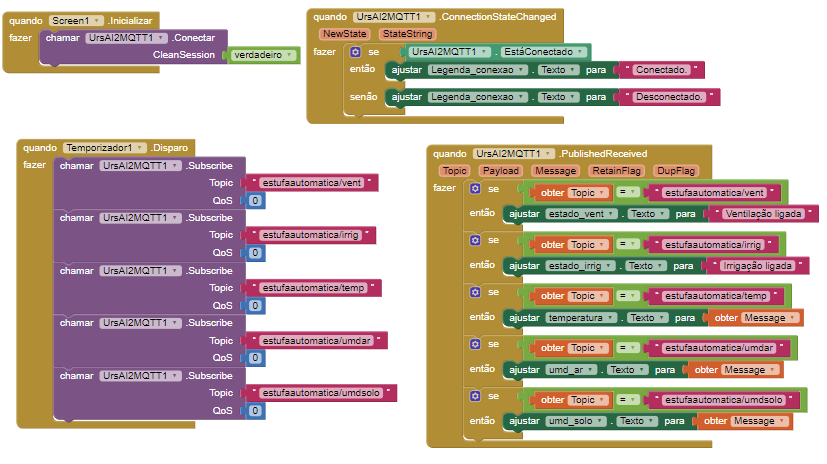
\includegraphics[width=12cm]{figuras/progbloco.png}\\
% 	\autoria{Autoria própria}
% 	\label{fig:progbloco}
% \end{figure}

% O aplicativo pode ser baixado gratuitamente pelo usuário através de link gerado durante o desenvolvimento do aplicativo, conforme mostrado na Figura \ref{fig:linkapk}. Foram adicionados na interface do aplicativo as mesmas informações que podem ser visualizadas pela interface humano/máquina física, no entanto, não permite realizar a configuração de escolha de plantio, sendo apenas possível ver a opção escolhida na IHM física. 

% \begin{figure}[!h]
% 	\centering
% 	\caption{Esquema de ligação do regulador de tensão}
% 	%\vskip 5mm
% 	
\includegraphics[width=12cm]{figuras/linkapk.png}\\
% 	\autoria{Autoria própria}
% 	\label{fig:linkapk}
% \end{figure}

% Conforme apresentado na Figura \ref{fig:apk}, o protótipo do aplicativo apresenta as principais informações do sistema de maneira simplificada, sendo de fácil manuseio e compreensão. 

% \begin{figure}[!h]
% 	\centering
% 	\caption{Interface do aplicativo de monitoramento}
% 	%\vskip 5mm
% 	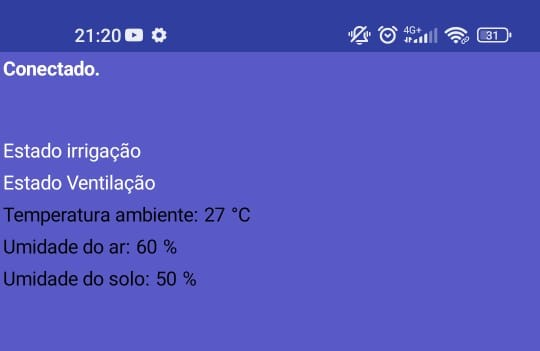
\includegraphics[width=10cm]{figuras/printapk.jpeg}\\
% 	\autoria{Autoria própria}
% 	\label{fig:apk}
% \end{figure}

% \subsection{Módulo central}

% O módulo central é responsável por intermediar a comunicação entre a \ac{IHM} e o circuito de condicionamento de sinais, tornando possível ao usuário o monitoramento remoto do sistema de irrigação, além de ser responsável por processar os comandos enviados pelo usuário. Esse módulo, apresentado na Figura \ref{fig:modcent}, é composto por placa ESP32, que faz a conexão com o servidor \ac{MQTT}, HC-12, que é utilizado para possibilitar a comunicação com o circuito de condicionamento. Esse módulo foi posicionado em localidade com acesso à internet, para possibilitar a conexão com a \ac{IHM}.

% \begin{figure}[!h]
% 	\centering
% 	\caption{Protótipo do módulo central}
% 	%\vskip 5mm
% 	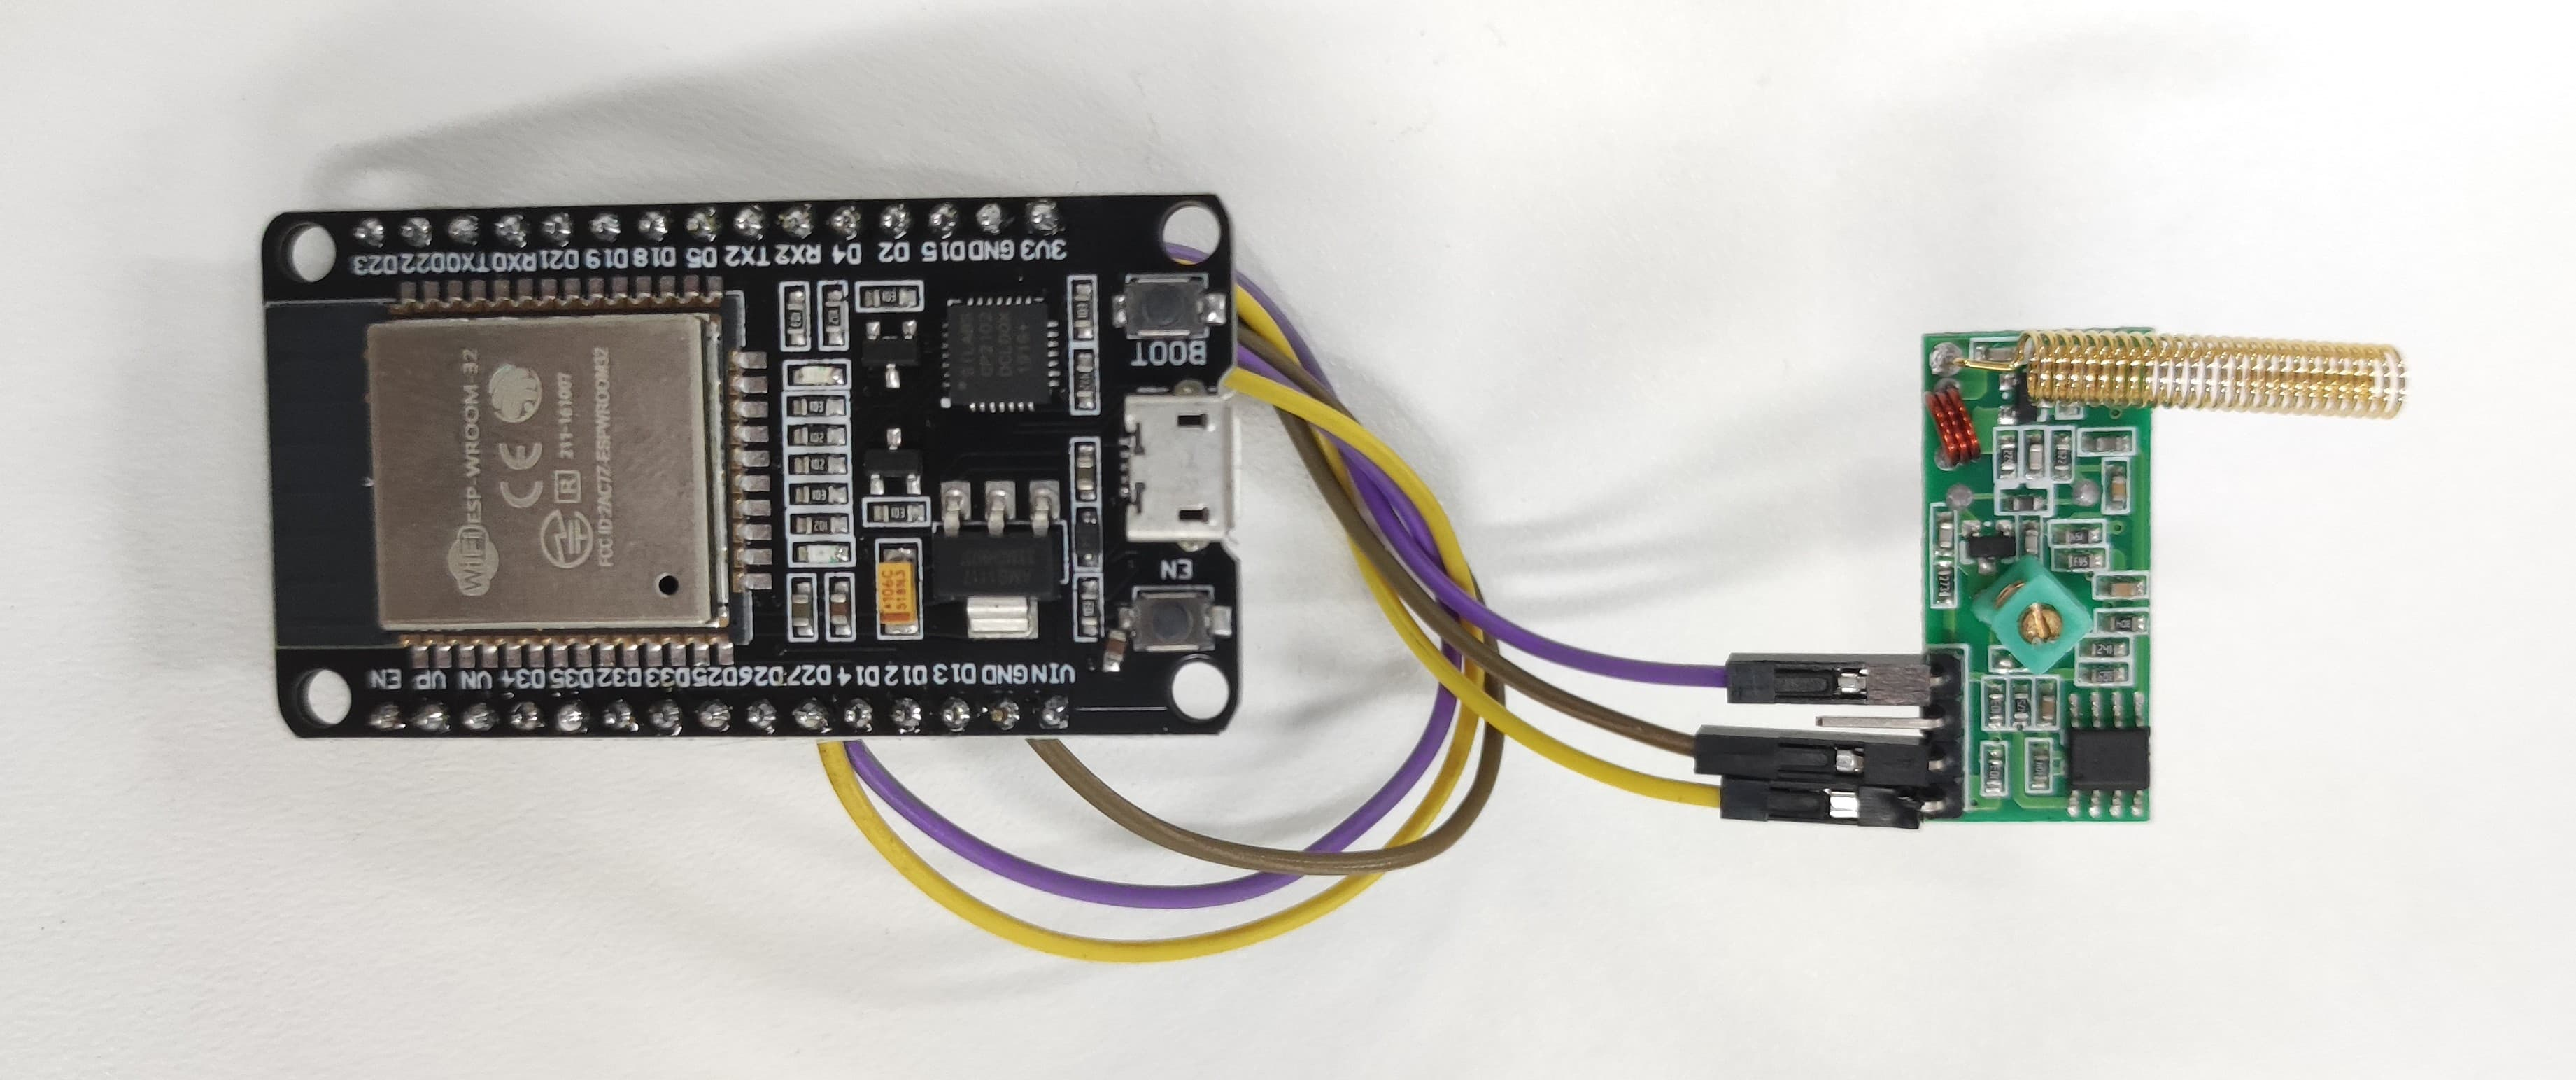
\includegraphics[width=10cm]{figuras/modcent.jpeg}\\
% 	\autoria{Autoria própria}
% 	\label{fig:modcent}
% \end{figure}

% \section{\textit{Software} embarcado}

% Neste trabalho, o \textit{Software} embarcado no microcontrolador foi desenvolvido com a linguagem C, utilizando a plataforma \textit{MikroC PRO for PIC} e a plataforma \textit{Arduíno IDE}. O fluxograma da Figura \ref{fig:alg} presenta de maneira simplificada o funcionamento da lógica de programação utilizada para o monitoramento e controle dos sistemas de ventilação e irrigação de uma estufa agrícola. 

% figura do fluxograma do software.
% \begin{figure}[!h]
% 	\centering
% 	\caption{Fluxograma do \textit{software} embarcado}
% 	%\vskip 5mm
% 	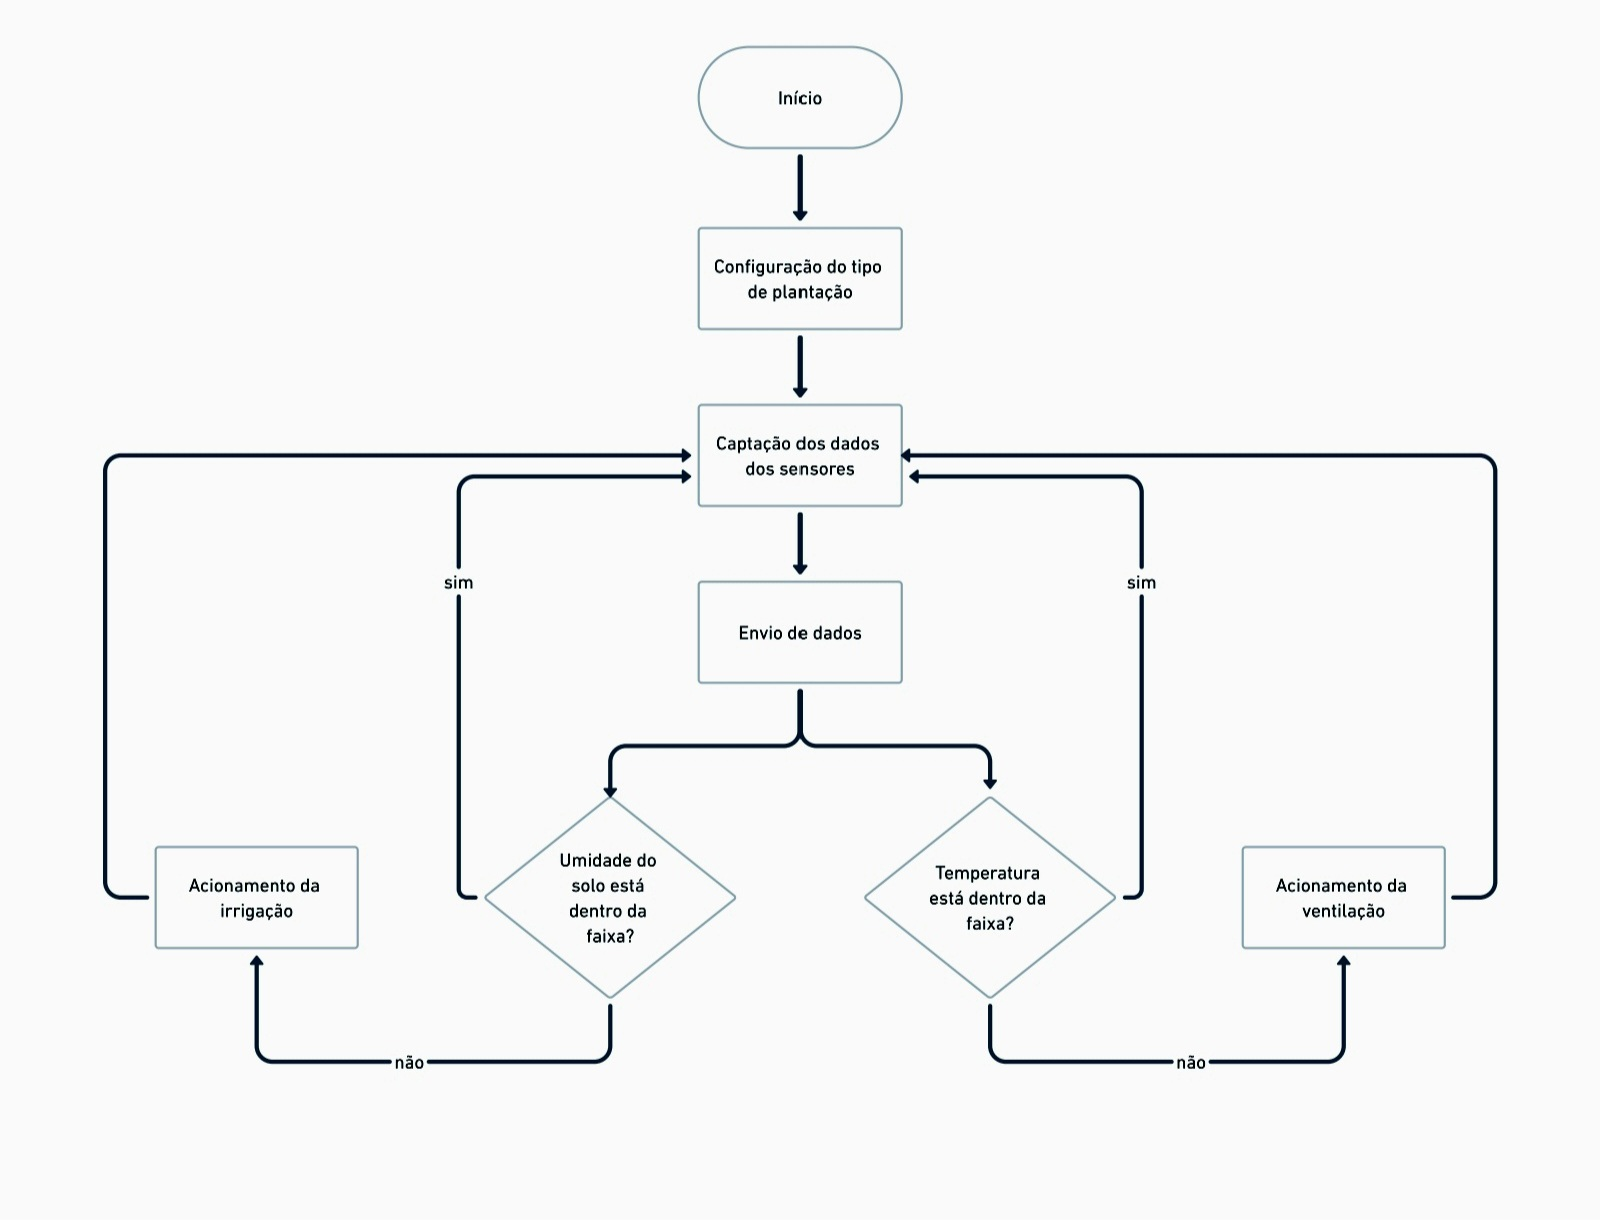
\includegraphics[width=12cm]{figuras/alg.jpg}\\
% 	\autoria{Autoria própria}
% 	\label{fig:alg}
% \end{figure}

% As principais etapas apresentadas no fluxograma são:
% \begin{enumerate}
%     \item Início: Inicializa o sistema com o carregamento das bibliotecas e a definição de variáveis e funções;
%     \item Configuração do tipo de plantação: Etapa em que o usuário escolhe o tipo de plantação que deseja aplicar o sistema, cada opção tem uma faixa de valores pré programados de temperatura e umidade do solo ideais para o plantio, essas faixas são informadas ao sistema após a escolha do usuário e passam a ser os parâmetros a serem alcançados pelo sistema;
%     \item Captação dos dados dos sensores: Nesta etapa o sistema coleta os dados dos sensores de umidade do solo, umidade relativa do ar e temperatura ambiente;
%     \item Envio de dados: Os dados coletados pelos sensores são enviados para a interface \textit{web}; 
%     \item Tomada de decisão: Caso o valor de temperatura ambiente não esteja dentro da faixa escolhida, a ventilação é acionada, os dados dos sensores são coletados novamente e uma nova tomada de decisão é realizada, o mesmo se aplica para a umidade do solo.
% \end{enumerate}   

% \subsection{Programação do sensor de temperatura e umidade do ar}

% O sensor DHT-22 possui uma programação complexa em comparação com outros sensores de temperatura, sendo dividida em funções que desempenham papeis diferentes em seu funcionamento, onde cada uma deve ser chamada no momento certo no código principal. Inicialmente foram definidas as portas onde o sensor foi conectado, em seguida foi definida a função de inicialização do sensor, chamada de \textit{start signal}, apresentada na Figura \ref{fig:startsig}.

% \begin{figure}[!h]
% 	\centering
% 	\caption{Função de inicialização do DHT-22}
% 	%\vskip 5mm
% 	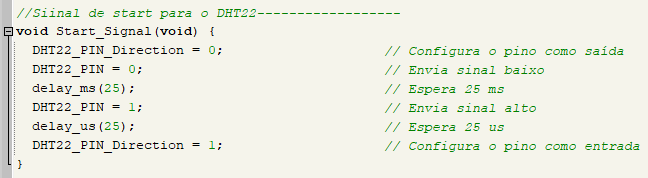
\includegraphics[width=12cm]{figuras/startsig.png}\\
% 	\autoria{Autoria própria}
% 	\label{fig:startsig}
% \end{figure}

% Essa função define o pino de conexão com o DHT-22 como saída e envia um pulso de nível lógico 1 por 20 ms, em seguida envia nível lógico 0 por 20ms, após isso o pino é definido como entrada e o sensor começa a enviar os dados. Em seguida, foi implementada a função que checa se a resposta do sensor apresenta algum erro, o código implementado é apresentado na Figura \ref{fig:chekres}. 

% \begin{figure}[!h]
% 	\centering
% 	\caption{Função de checagem da resposta do DHT-22}
% 	%\vskip 5mm
% 	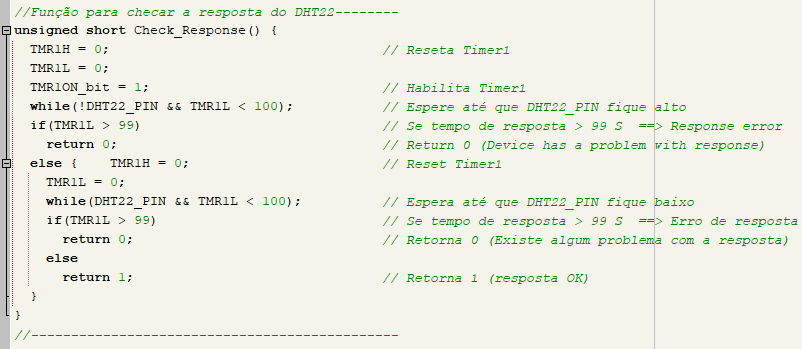
\includegraphics[width=12cm]{figuras/chekres.png}\\
% 	\autoria{Autoria própria}
% 	\label{fig:chekres}
% \end{figure}

% Essa função verifica a quantidade de bits recebidos do sensor e compara com o padrão de envio, que são 16 bits, caso encontre erro a função exibe a mensagem de erro na tela, caso contrario, da prosseguimento ao código. Seguindo para a função principal, ocorre a separação dos bits de umidade relativa do ar e os de temperatura ambiente, que são convertidos em valores decimais, que por sua vez, são usados para a tomada de decisão e exibidos ao usuário, conforme é visto na Figura \ref{fig:lerdados}.

% \begin{figure}[!h]
% 	\centering
% 	\caption{Função de leitura de dados do DHT-22}
% 	%\vskip 5mm
% 	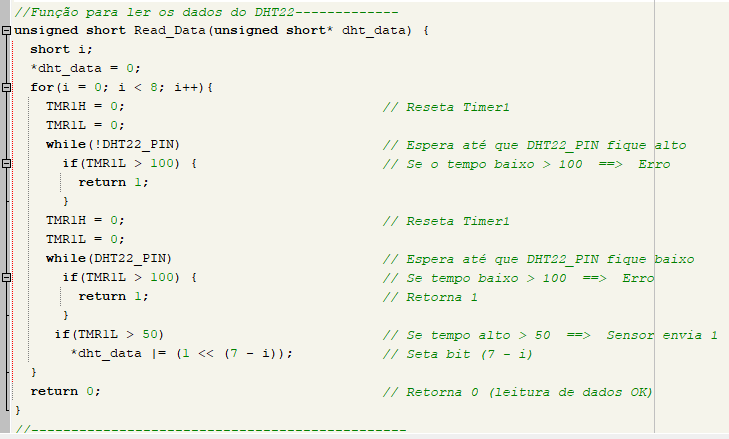
\includegraphics[width=12cm]{figuras/lerdados.png}\\
% 	\autoria{Autoria própria}
% 	\label{fig:lerdados}
% \end{figure}

% \subsection{Programação do sensor de umidade do solo}

% A programação referente ao sensor de umidade do solo é mais simples, visto que é enviado um valor analógico de tensão variando entre 0 a 5V, que é convertido pelo microcontrolador para um valor entre 0 a 1023, por conta do conversor analógico/digital do PIC18F4550 ser composto por 8 bits. Então, esse número é convertido para um valor entre 0 a 100\%, conforme apresentado na Figura \ref{fig:codsolo}, que corresponde à umidade do solo. 

% \begin{figure}[!h]
% 	\centering
% 	\caption{Função de leitura do sensor de umidade do solo}
% 	%\vskip 5mm
% 	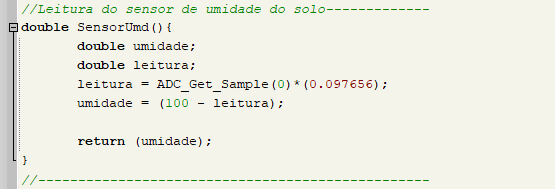
\includegraphics[width=12cm]{figuras/codsolo.png}\\
% 	\autoria{Autoria própria}
% 	\label{fig:codsolo}
% \end{figure}

% \subsection{Programação dos atuadores}

% Para o acionamento dos atuadores, foram desenvolvidas duas funções distintas, porém, com funcionamento parecidos. As funções recebem as faixas de valores ideais para o plantio escolhido pelo usuário, em seguida recebem os valores lidos pelos sensores. Para o acionamento da ventilação, a função compara os dados do sensor de temperatura com o valor programado, caso a temperatura esteja dentro da faixa, a função desliga a ventilação, caso esteja maior, a função liga a ventilação, conforme visto na Figura \ref{fig:codvent}.

% \begin{figure}[!h]
% 	\centering
% 	\caption{Função de acionamento da ventilação}
% 	%\vskip 5mm
% 	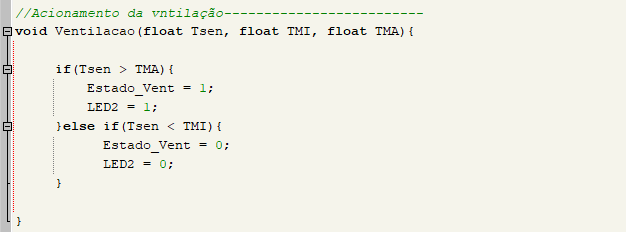
\includegraphics[width=12cm]{figuras/codvent.png}\\
% 	\autoria{Autoria própria}
% 	\label{fig:codvent}
% \end{figure}

% A função de acionamento da irrigação compara os dados do sensor de umidade do solo com a faixa de valores programados. Todavia, foi implementado um intervalo de histerese, para que não ocorra o acionamento e desacionamento desnecessário da irrigação, visto que os valores de umidade podem oscilar entre o limite do valor ideal conforme exibido na Figura \ref{fig:codirrig}.

% \begin{figure}[!h]
% 	\centering
% 	\caption{Função de acionamento da irrigação}
% 	%\vskip 5mm
% 	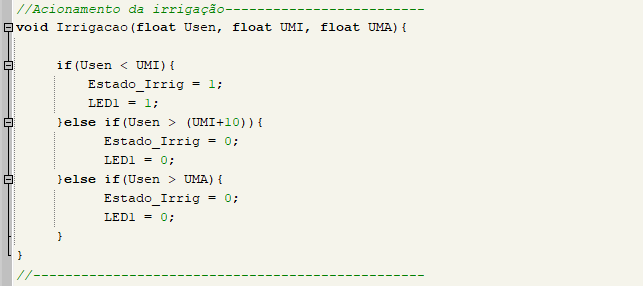
\includegraphics[width=12cm]{figuras/codirrig.png}\\
% 	\autoria{Autoria própria}
% 	\label{fig:codirrig}
% \end{figure}

% \section{Custo do sistema}

% O protótipo foi desenvolvido visando manter um custo baixo, em comparação aos produtos de automação de irrigação encontrados no mercado, para que possa ser acessível aos agricultores familiares e pequenos produtores. Desse modo, foram realizadas buscas pelos melhores preços para os componentes utilizados no projeto, a Tabela \ref{tab:custo} apresenta a relação de custo dos principais componentes do trabalho.

% \begin{table}[!h]
% \centering
% \caption{Custo do sistema}
% \label{tab:custo}
% \begin{tabular}{l|c|c|c}
% \hline
% Componente & \multicolumn{1}{l|}{Custo unitário (R\$)} & \multicolumn{1}{l|}{Quantidade (un)} & \multicolumn{1}{l}{Custo total (R\$)} \\ \hline
% Placa microStart & 60,00 & 1 & 60,00 \\ \hline
% Módulo Relé & 34,00 & 1 & 34,00 \\ \hline
% Esp32 & 38,90 & 1 & 22,90 \\ \hline
% Display LCD & 16,95 & 1 & 16,95 \\ \hline
% DHT-22 & 20,42 & 1 & 20,42 \\ \hline
% HD-38 & 9,32 & 1 & 9,32 \\ \hline
% HC-12 & 9,98 & 2 & 19,96 \\ \hline
% Insumos & 20,00 & 1 & 20,00 \\ \hline
% Caixa & 36,45 & 1 & 36,45 \\ \hline
% \textbf{Custo total} & - & - & \textbf{240,00} \\ \hline
% \end{tabular}
% \\
% \autoria{Autoria própria}
% \end{table}

% Insumos como resistores, diodos emissores de luz, botões, fios e cabos, placa de fenolite, capacitores e parafusos foram utilizados do próprio autor, sendo estimados em R\$ 20,00 reais. Por serem materiais com custo baixo em comparação aos principais componentes do sistema, essa estimativa não impacta significativamente na fidelidade do custo total do sistema implementado. 

% Foram realizadas pesquisas em lojas de agricultura na região de Irecê, para realizar uma comparação com um sistema comercial com características compatíveis com o protótipo, porém, apenas um sistema de automação de irrigação foi encontrado. O sistema não possui sensores de temperatura e umidade do solo, sendo controlado apenas válvulas solenoides para o controle de bombeamento de água, contando com divisão em diferentes setores. A programação a ser realizada também é mais complexa que o protótipo desenvolvido no presente trabalho, se tornando mais difícil de manusear, na Tabela \ref{tab:comp} é realizada uma comparação entre funcionalidades e custo do sistema comercial Irriplus VR e o sistema desenvolvido nesse trabalho.

% \begin{table}[!h]
% \centering
% \caption{Comparação entre os sistemas }
% \label{tab:comp}
% \begin{tabular}{l|c|c}
% \hline
% Funções & \begin{tabular}[c]{@{}c@{}}Protótipo \\ desenvolvido\end{tabular} & \begin{tabular}[c]{@{}c@{}}Irriplus \\ VR\end{tabular} \\ \hline
% \begin{tabular}[c]{@{}l@{}}Monitoramento de\\ temperatura\end{tabular} & SIM & NÃO \\ \hline
% \begin{tabular}[c]{@{}l@{}}Monitoramento de \\ umidade do ar\end{tabular} & SIM & NÃO \\ \hline
% \begin{tabular}[c]{@{}l@{}}Monitoramento de \\ umidade do solo\end{tabular} & SIM & NÃO \\ \hline
% Controle de irrigação & SIM & SIM \\ \hline
% Controle de ventilação & SIM & NÃO \\ \hline
% Divisão por setores & NÃO & SIM \\ \hline
% \begin{tabular}[c]{@{}l@{}}Monitoramento \\ remoto\end{tabular} & SIM & NÃO \\ \hline
% \textbf{Custo R\$} & 240,00 & 1529,86 \\ \hline
% \end{tabular}
% \\
% \autoria{Autoria própria}
% \end{table}

% Mesmo com custo quase seis vezes menor, o sistema desenvolvido se mostrou mais completo, tendo maior controle das variáveis que envolvem a irrigação, sendo uma boa opção para a agricultura familiar e também para grandes produtores.

% \section{Requisitos do sistema}

% Para determinar os requisitos que o trabalho deve atender, é necessário analisar os principais cultivos a serem implementados em estufas, buscando suas condições ideais de temperatura, umidade do solo e umidade relativa do ar. As cultivares predominantes em estufas são hortaliças, plantas hidropônicas e frutíferas, que apresentam necessidades semelhantes quanto ao clima, sendo possível estabelecer intervalos de valores que atendam a essas características.

% A temperatura ideal de cultivo de grande parte das plantas hidropônicas é de 25°C, para morangos e frutas semelhantes, é estabelecido um intervalo entre 15°C e 25°C para um bom desenvolvimento dos frutos, a temperatura ótima para e cultivo de cenouras e outras raízes tuberosas varia entre 20°C e 30°C. Com isso, compreende-se que o protótipo deve ser capaz de mensurar valores de temperatura compreendidos entre 15°C e 30°C para a maioria das plantações, contudo, para que o sistema possa quantificar também a variação de temperatura ambiente e com isso tomar melhores decisões de controle considerando a variação climática das diversas regiões do Brasil, a faixa de valores que deve ser medida compreende entre -15°C e 50°C.

% Para a umidade do solo os valores ideais dependem não apenas da variedade de cultivo, como também do tipo de solo. Contudo, a gama ideal de teor de umidade do solo para a maioria das culturas está entre 20\% e 60\%. É crucial para o bom funcionamento do sistema que o protótipo seja capaz de medir valores que estejam fora da faixa ideal de cultivo, para que o controle tome a decisão apropriada para a situação. Destarte, os valores a serem mensurados estarão entre 5\% e 95\%.

% Altos níveis de umidade relativa do ar geram condições favoráveis para o surgimento e proliferação de doenças nas plantas. Em contrapartida, níveis muito baixos podem ocasionar ressecamento no cultivo. A faixa a ser monitorada pelo sistema está compreendida entre 0 a 100\%. A Tabela \ref{tab:my-tablex} apresenta os valores a serem medidos como requisitos do sistema.

% \begin{table}[!h]
% \centering
% \caption{Parâmetros a serem medidos.
% }
% \label{tab:my-tablex}
% \begin{tabular}{c|c|c}
% \hline
% \textbf{Descrição}       & \textbf{Min}   & \textbf{Max}   \\ \hline
% {Temperatura}     & {-15°C} & {50°C}  \\ \hline
% {Umidade do solo} & {5\%}   & {95\%}  \\ \hline
% {Umidade do ar}   & {0\%}   & {100\%} \\ \hline
% \end{tabular}
% \\
% \autoria{Autoria própria}
% \end{table}

% %\section{Ferramentas computacionais utilizadas}



% \section{Metodologia de avaliação dos resultados}

% A avaliação dos resultados foi embasada nos objetivos do projeto e nos requisitos do sistema. Os módulos do sistema foram avaliados de acordo com a sua funcionalidade. Para o módulo de sensores foram avaliados a confiabilidade dos dados coletados, comparando-os com os valores reais, para isso foram realizados testes em ambiente controlado, para os atuadores foram verificados o tempo de resposta e a reação aos comandos enviados pelo módulo central.

% Para avaliar o envio de dados, foram levados em consideração a segurança da conectividade entre os módulos, além do alcance da conexão. Esses fatores são importantes para avaliar se o projeto é resistente à perdas de conexão e corrompimento dos dados transmitidos. Foram realizados testes variando-se a distancia entre os módulos, enviando dados conhecidos e comparando-os com a resposta obtida nos demais módulos. A \ac{IHM} deve ter uma interface amigável e intuitiva ao usuário, livre de erros de programação e travamentos. 





